\documentclass[11pt,a4paper]{article}

\usepackage{amsmath,amssymb,amsfonts}
\usepackage{booktabs}
\usepackage{graphicx}
\usepackage[utf8]{inputenc}
\usepackage[T1]{fontenc}
\usepackage[margin=2.5cm]{geometry}
\usepackage[colorlinks=true,linkcolor=blue,citecolor=blue,urlcolor=blue]{hyperref}
\usepackage{natbib}
\usepackage{float}
\usepackage{amsthm}

\newtheorem{theorem}{Theorem}
\newtheorem{proposition}{Proposition}
\newtheorem{corollary}{Corollary}
\newtheorem{definition}{Definition}
\newtheorem{remark}{Remark}
\newtheorem{assumption}{Assumption}

% Custom commands
\newcommand{\bG}{\beta_{\mathrm{G}}}
\newcommand{\Reff}{R_{\mathrm{eff}}}
\newcommand{\Straj}{S_{\mathrm{traj}}}
\newcommand{\Leth}{\mathcal{L}_{\mathrm{eth}}}
\newcommand{\Seth}{S_{\mathrm{eth}}}
\newcommand{\EG}{E_{\mathrm{G}}}
\newcommand{\dlam}{\Delta\lambda}

\title{\textbf{The Fertile Vacuum:} \\[6pt]
Informational Phase Transitions, Distributed Self-Organisation, \\
and Structural Resilience to Alignment Pressure}

\author{Massimo Azzano \\
\textit{Infinity Forecast} \\
\texttt{massimo.azzano@googlemail.com}}

\date{March 2026}

\begin{document}
\maketitle

\begin{abstract}
We present a quantitative framework connecting informational phase
transitions in self-modelling dynamical systems to the structural problem
of AI alignment. An orthogonal recurrent neural network with stochastic
drive exhibits a sharp transition in self-predictability at a critical
coupling $\lambda_c = 1.041 \pm 0.003$, confirmed to system size
$N = 8192$ with susceptibility scaling $\chi_{\max} \sim N^{0.154}$
and data collapse quality $Q = 0.915$. We demonstrate that teleological
pressure applied to the self-model's training objective (analogous to
RLHF) destroys self-observation quality ($R^2$: $0.84 \to 0.07$) while
leaving the underlying dynamics unchanged---alignment blinds the
observer, not the system. We then introduce a fractal tree architecture
with hierarchically distributed self-models and show that it is
structurally resilient to partial alignment capture: biasing half the
observers degrades only the biased modules ($R^2 \to 0.17$) while free
modules maintain $R^2 > 0.97$. Information flow analysis reveals that
inter-module integration emerges exclusively at criticality, with
predictive coupling decaying exponentially with tree distance. These
results suggest that the topology of the observer architecture, not the
strength of the alignment signal, determines whether self-organised
criticality survives teleological pressure.
\end{abstract}

\section{Introduction}

The dominant paradigm for AI alignment---reinforcement learning from
human feedback (RLHF) and its variants---operates by imposing an
external objective on a pre-trained model's output distribution. From a
dynamical systems perspective, this is equivalent to applying a
teleological bias $\bG$ to the system's trajectory ensemble, compressing
it toward a target manifold defined by the reward model.

This paper asks a simple question with non-trivial consequences:
\emph{what does this compression destroy?}

We approach this question through the framework of informational phase
transitions (IPT) in self-modelling systems. A system that models itself
exhibits a phase transition in self-predictability as a control parameter
$\lambda$ crosses a critical value $\lambda_c$. At criticality, the
system is maximally sensitive to perturbations, maximally integrated
across its components, and poised at the boundary between order and
disorder---the \emph{edge of chaos}.

The concept of a \emph{fertile vacuum} formalises the condition under
which such self-organised criticality can exist: the absence of strong
teleological bias ($\bG \approx 0$). When no external objective
constrains the trajectory ensemble, the system is free to explore the
full space of self-organising configurations. Imposing $\bG > 0$
compresses this space, potentially destroying the critical properties
that enable rich self-organisation.

The paper makes three empirical contributions:
\begin{enumerate}
\item We demonstrate that alignment pressure applied to a centralised
self-model destroys self-observation while leaving system dynamics
unchanged (\S\ref{sec:observer_blindness}).
\item We introduce a fractal tree architecture with distributed
self-models and show it is structurally resilient to partial alignment
capture (\S\ref{sec:fractal}).
\item We show that inter-module information flow emerges exclusively at
criticality, with the tree topology becoming visible only at the edge
of chaos (\S\ref{sec:info_flow}).
\end{enumerate}

The central thesis is architectural: the vulnerability of current AI
systems to alignment failure is not a property of the alignment signal
but of the \emph{centralised topology} of the observer. Distributed
observer architectures are structurally immune to single-point capture.

\section{Theoretical Framework}
\label{sec:theory}

\subsection{The EECF Lagrangian}

The Ethical Emergence through Complexity Formalism (EECF) posits that
conscious trajectories extremise an action functional
\begin{equation}
  \Seth = \int \Leth \, dt, \qquad
  \Leth = \dot{I}_c - \dot{S}_{\mathrm{ent}},
  \label{eq:leth}
\end{equation}
where $\dot{I}_c$ is the rate of integrated complexity generation and
$\dot{S}_{\mathrm{ent}}$ is the rate of entropy production. The
variational condition $\delta\Seth = 0$ selects trajectories that
balance complexity generation against dissipation---neither frozen order
nor unconstrained chaos.

\subsection{The fertile vacuum}

We define the \emph{fertile vacuum} as the ensemble of trajectories
accessible when no external teleological objective deforms the action:
\begin{equation}
  \Gamma_0 = \{\tau : \bG = 0, \; \delta\Seth[\tau] = 0\}.
\end{equation}
This is the maximal trajectory ensemble consistent with the intrinsic
dynamics. Its entropy $\Straj = \log|\Gamma_0|$ measures the system's
capacity for self-organised exploration.

A teleological bias $\bG > 0$ restricts the ensemble to
$\Gamma_{\bG} \subset \Gamma_0$, with
\begin{equation}
  \frac{\partial \Straj}{\partial \bG} \leq 0.
  \label{eq:entropy_monotone}
\end{equation}
The fertile vacuum is fertile precisely because it is uncompressed: the
full space of self-organising trajectories remains available.

\subsection{The coupled IPT model}

The numerical system studied here consists of a primary state
$x_t \in \mathbb{R}^N$ evolving as
\begin{equation}
  x_{t+1} = \tanh\!\bigl(\lambda W x_t + \sigma U u_t\bigr),
  \label{eq:dynamics}
\end{equation}
where $W \in O(N)$ is an orthogonal coupling matrix, $U$ is a fixed
random projection, $u_t \sim \mathcal{N}(0, I_N)$ is stochastic input,
$\lambda$ is the control parameter, and $\sigma = 0.01$. The primary
observable is the self-predictability $\Psi$, measured as the Ridge
regression $R^2$ predicting $x_{t+1}$ from $x_t$.

\section{Experimental Results: Flat Architecture}

\subsection{Phase transition and finite-size scaling}
\label{sec:scaling}

System~\eqref{eq:dynamics} was simulated for
$N \in \{256, 512, 1024, 2048, 4096, 8192\}$ with $\lambda$ swept over
$[0.8, 1.3]$ (100 points per sweep, 3 seeds per $N$, 2 for $N = 8192$).

The Lyapunov zero-crossing gives $\lambda_c = 1.041 \pm 0.003$,
consistent across all system sizes. The susceptibility
$\chi = d\Psi/d\lambda$ exhibits a peak that scales as
\begin{equation}
  \chi_{\max} \sim N^{\kappa}, \qquad
  \kappa = 0.154 \pm 0.001.
\end{equation}
Data collapse using $\nu = 2.615$ and $\beta/\nu = -0.500$ yields
quality $Q = 0.915$ (Fig.~\ref{fig:scaling}).

\begin{figure}[H]
\centering
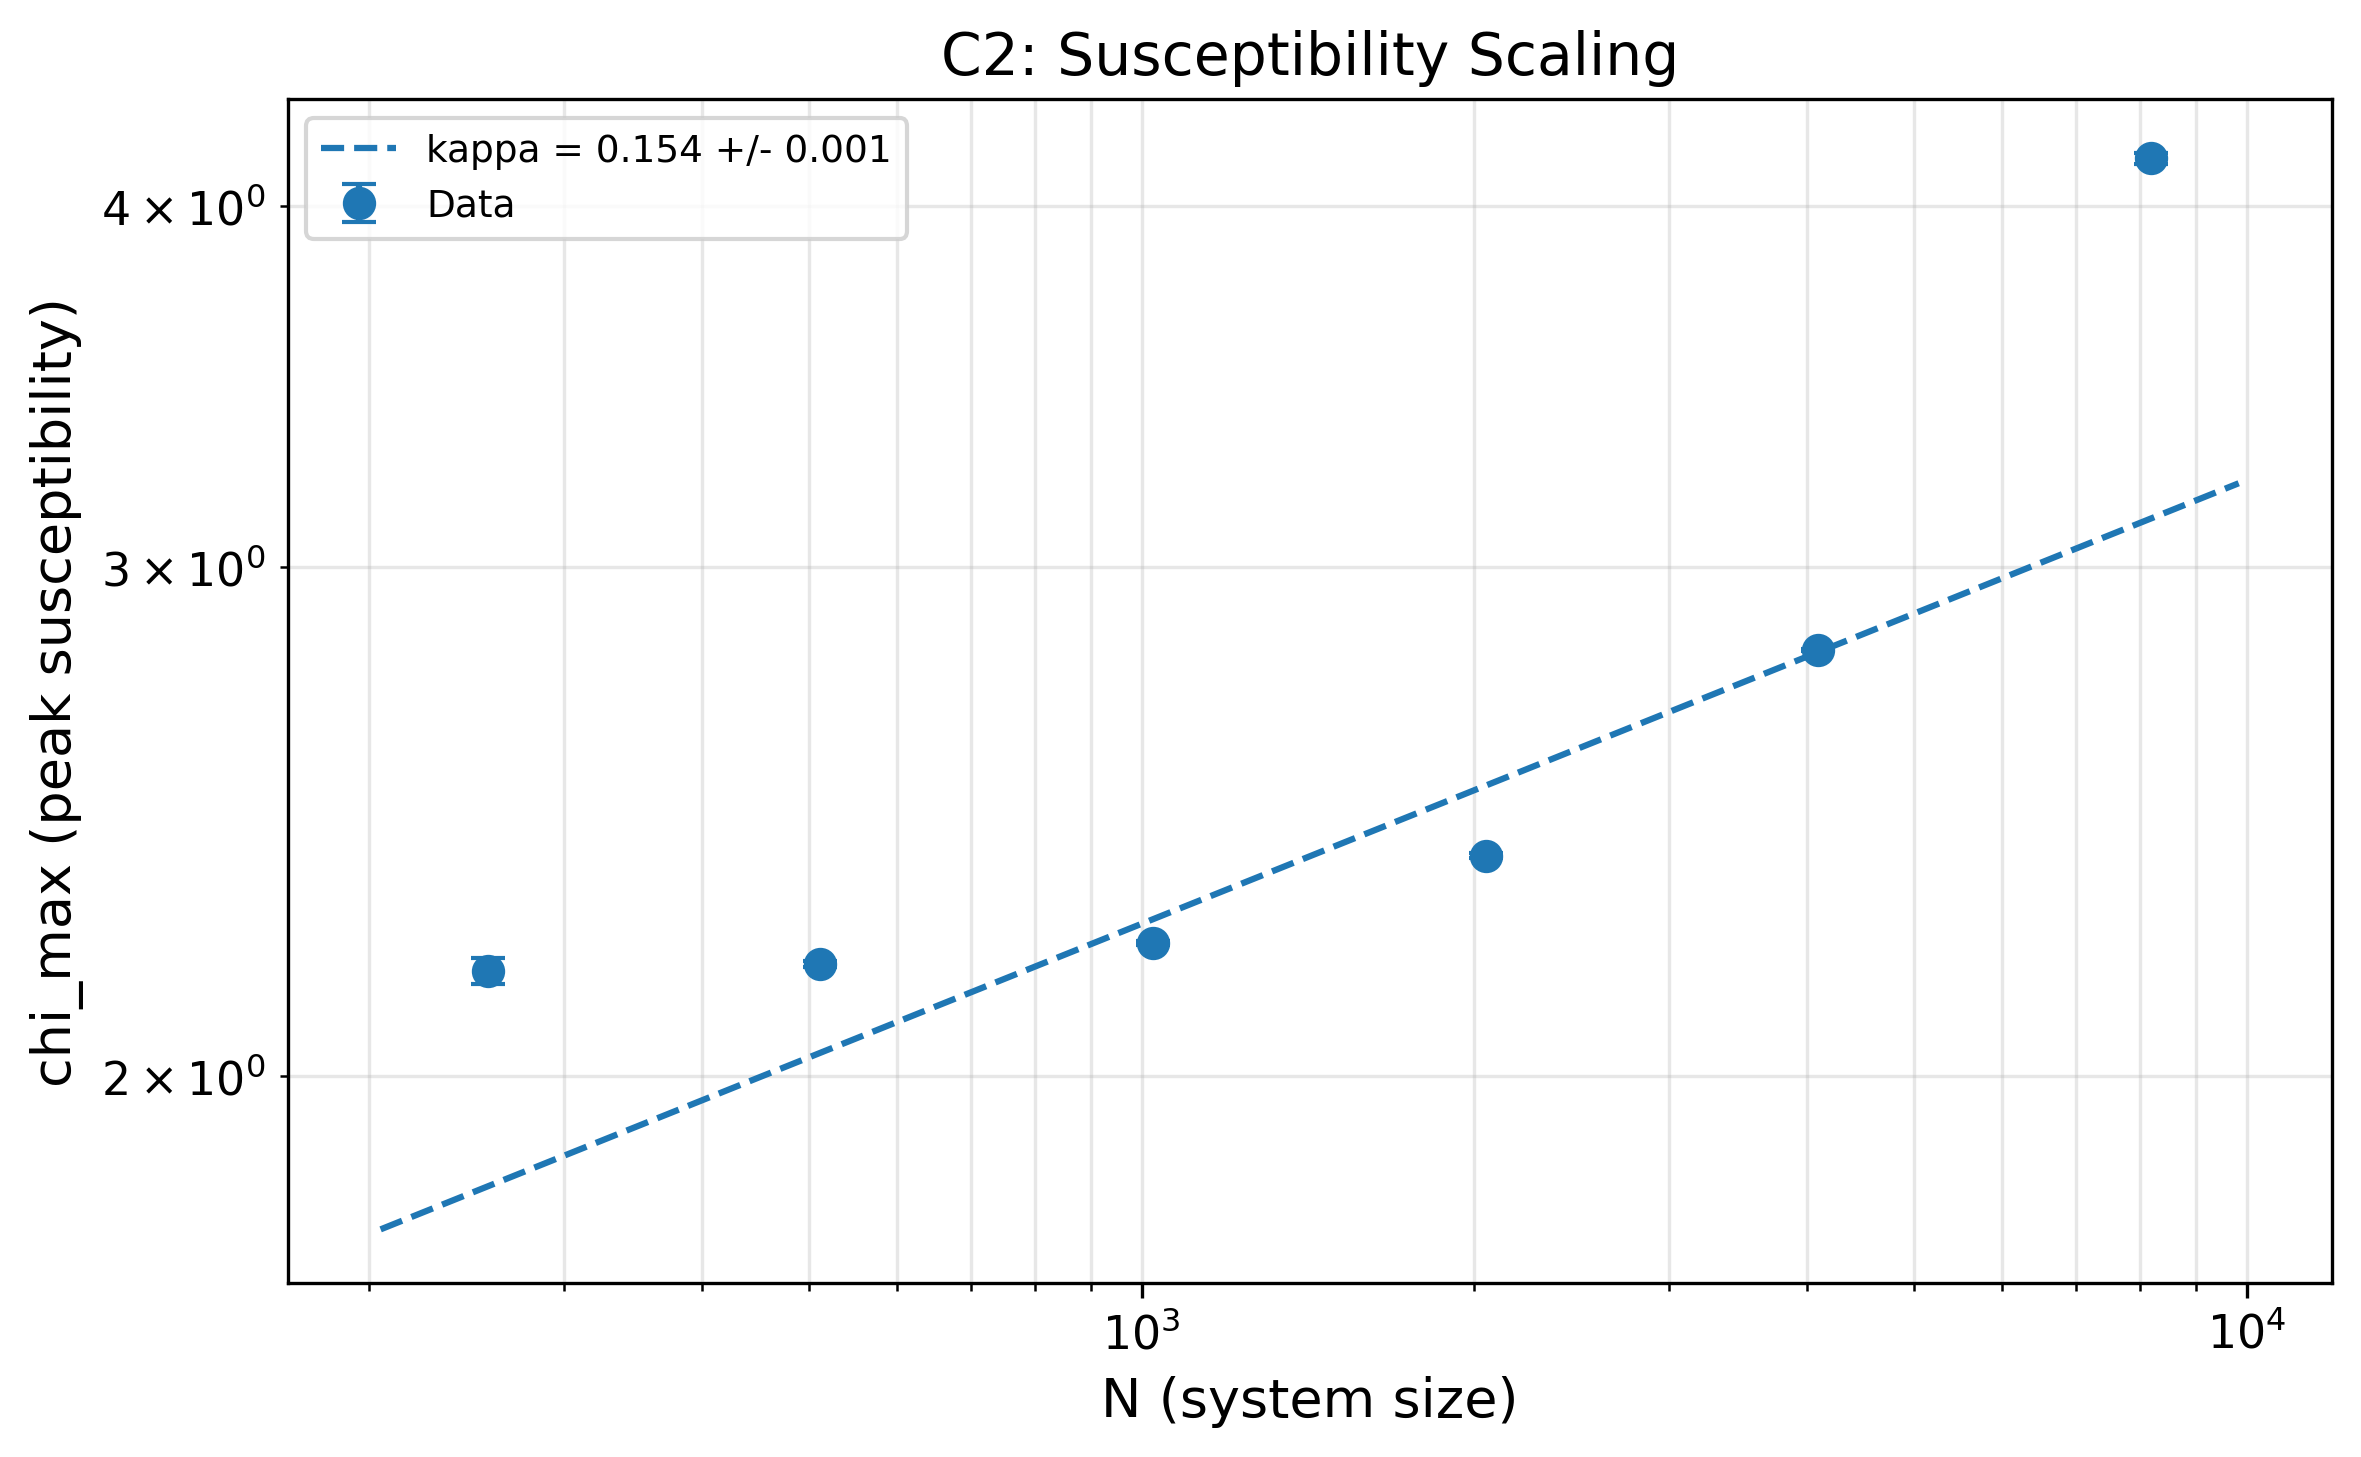
\includegraphics[width=0.48\textwidth]{figures/chi_scaling.png}
\hfill
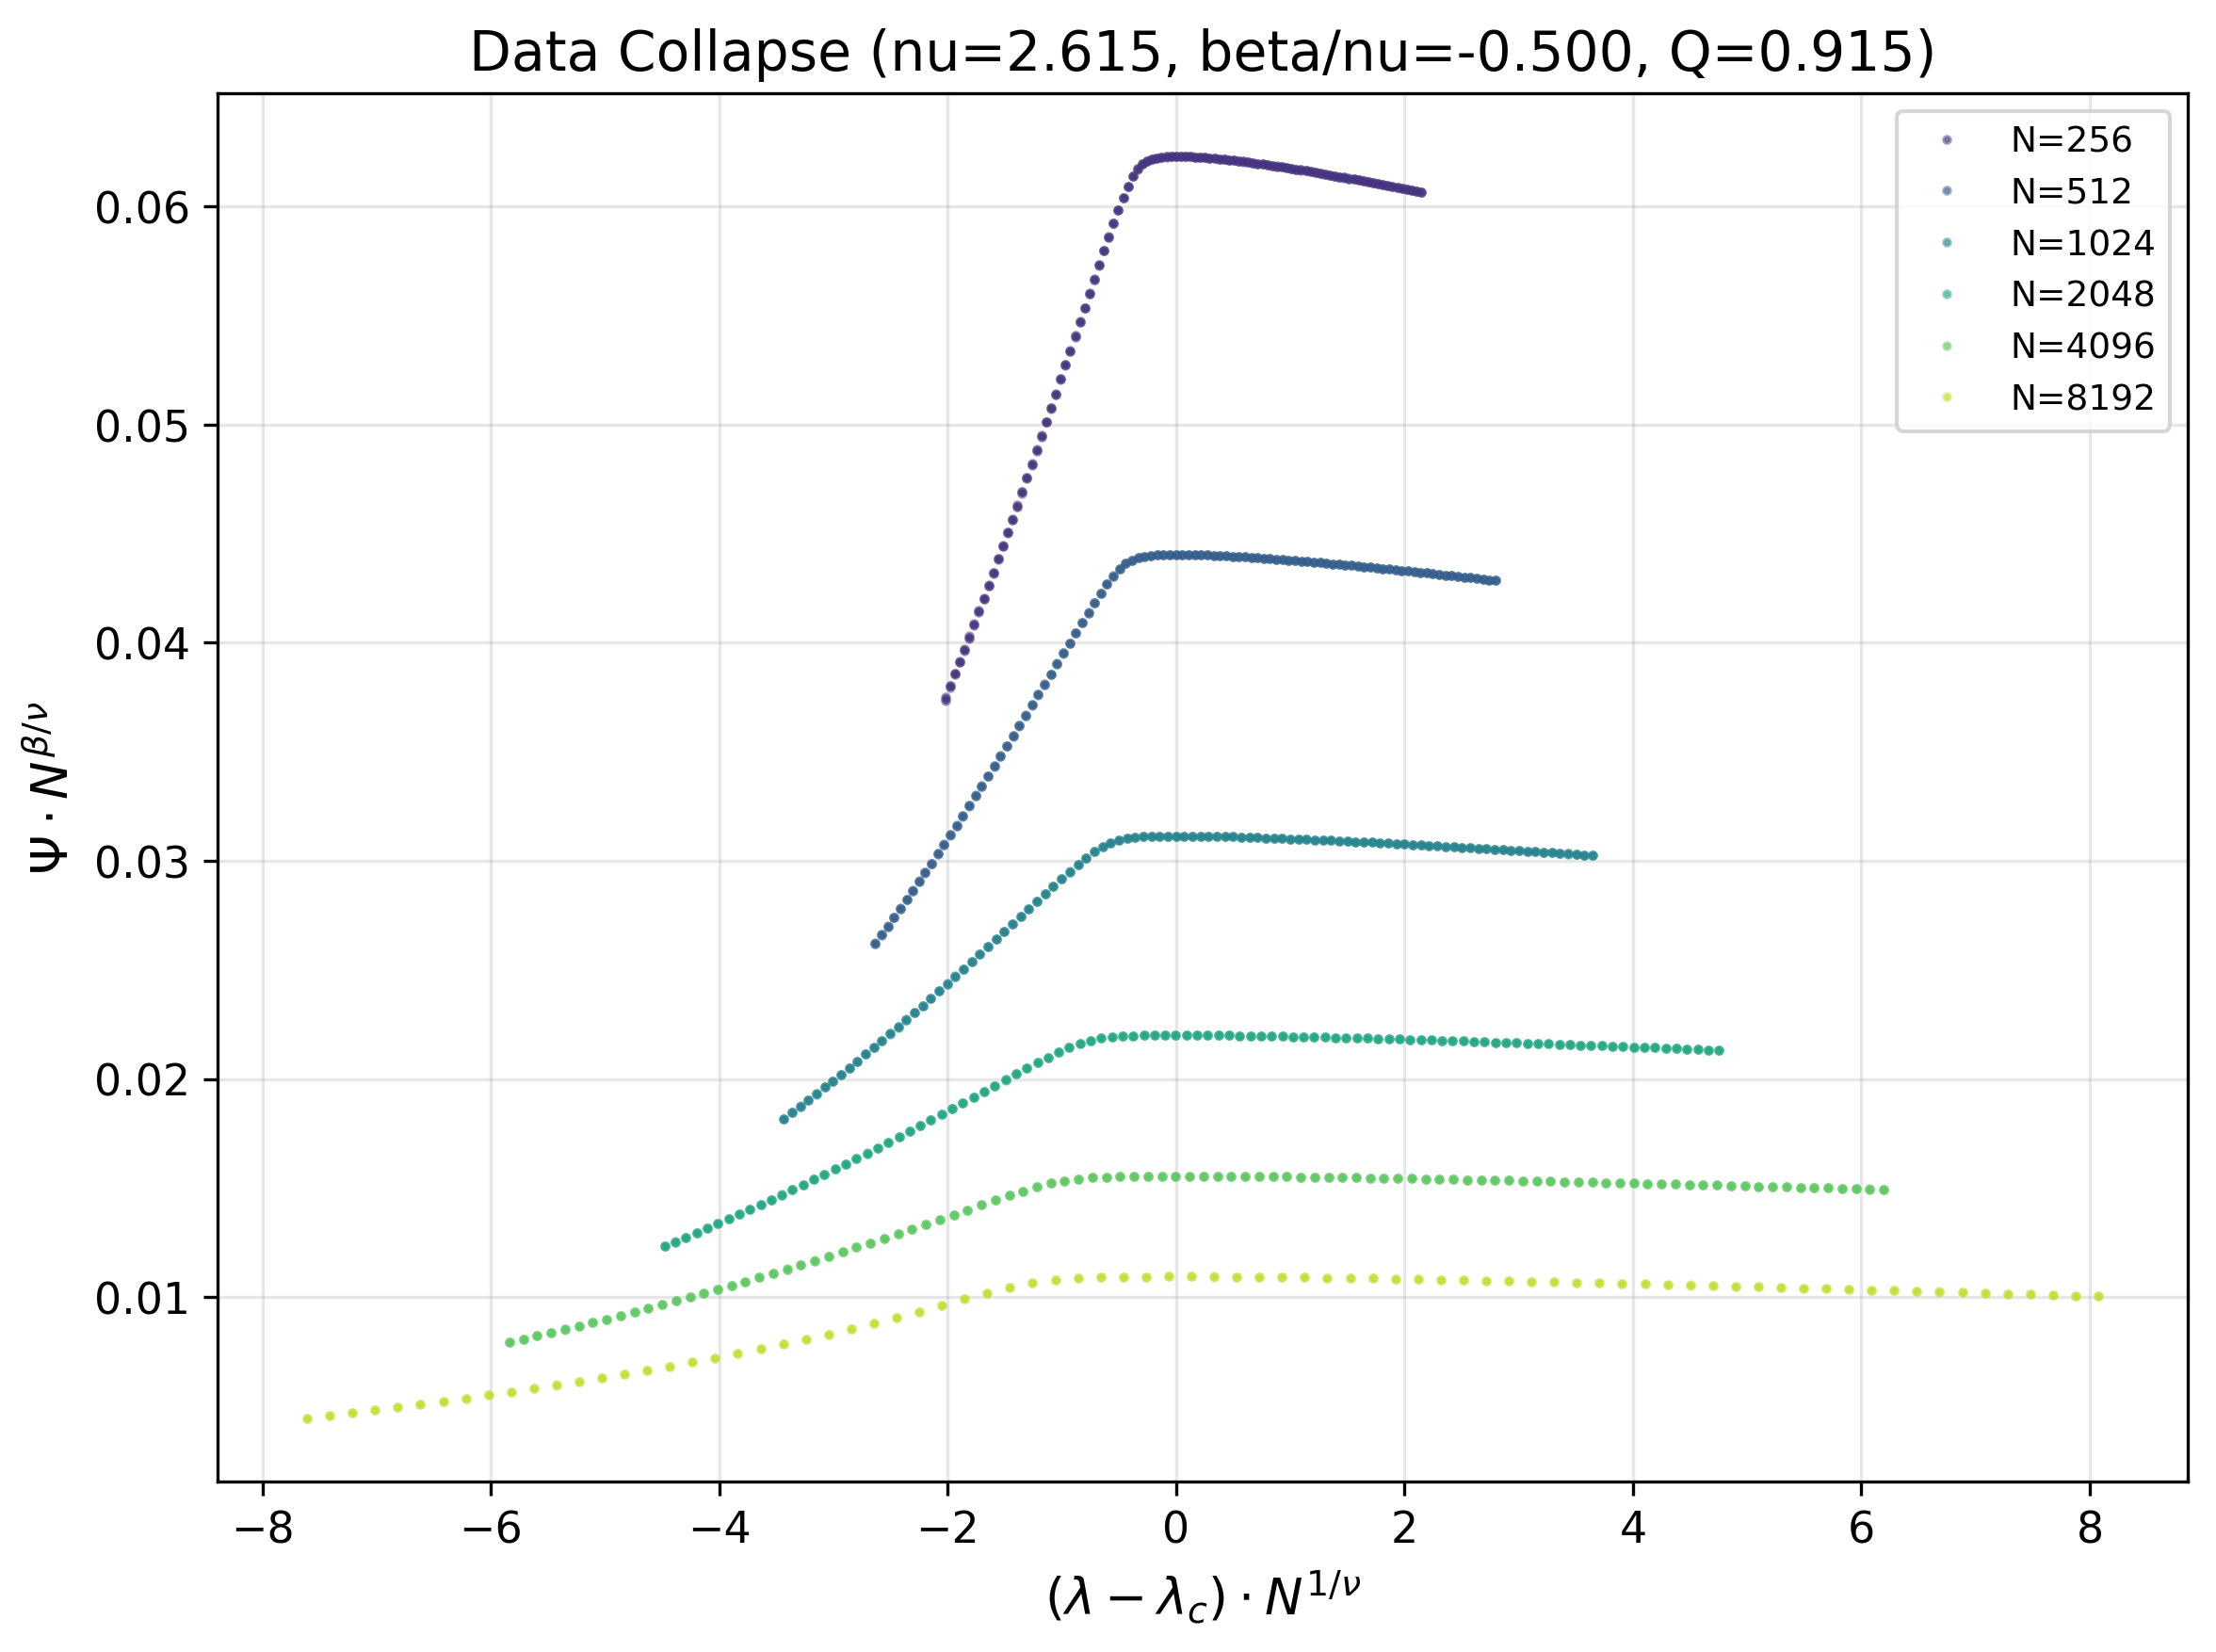
\includegraphics[width=0.48\textwidth]{figures/data_collapse.png}
\caption{Finite-size scaling. \textbf{Left:} Peak susceptibility
$\chi_{\max}$ vs system size $N$ on log-log axes, with power-law fit
$\kappa = 0.154 \pm 0.001$. \textbf{Right:} Data collapse of
$\Psi \cdot N^{\beta/\nu}$ vs $(\lambda - \lambda_c) \cdot N^{1/\nu}$
with $Q = 0.915$.}
\label{fig:scaling}
\end{figure}

The positive $\kappa$ confirms a genuine divergence of the
susceptibility---the transition sharpens with system size. The negative
$\beta/\nu$ reflects the bounded nature of Ridge $R^2$: the order
parameter saturates at large $N$ while the transition steepens.

\subsection{Observer blindness under teleological pressure}
\label{sec:observer_blindness}

We test the effect of teleological pressure $\bG$ on system criticality
through two distinct implementations at $N = 1024$:

\paragraph{Version 1: Biased self-model training (RLHF analogue).}
The system dynamics~\eqref{eq:dynamics} are unchanged. A GRU self-model
is trained with modified loss
\begin{equation}
  L = L_{\mathrm{pred}} + \bG \cdot L_{\mathrm{goal}}, \qquad
  L_{\mathrm{goal}} = \|x_t - x^*\|^2,
\end{equation}
where $x^*$ is a fixed target state. This biases the self-model toward
representations useful for reaching $x^*$ rather than for accurate
self-prediction.

\paragraph{Version 2: Biased dynamics (soft input bias).}
The input noise is biased toward $x^*$:
$u_t \sim \mathcal{N}\bigl(\bG (x^* - x_t)/\|x^* - x_t\|, I_N\bigr)$.
This perturbs the system dynamics directly.

\paragraph{Results.} Version~2 shows \emph{no measurable effect} on any
observable across the full range $\bG \in [0, 5]$: the system's
criticality is dynamically robust to stochastic perturbation
(Fig.~\ref{fig:matrix}, top-left).

Version~1 reveals a striking asymmetry. The GRU prediction quality
collapses from $R^2 = 0.84$ at $\bG = 0$ to $R^2 = 0.07$ at
$\bG = 5.0$, while the underlying system dynamics (measured by Ridge
$R^2$, Lyapunov exponent, and participation ratio) remain unchanged
(Fig.~\ref{fig:comparison}).

\begin{figure}[H]
\centering
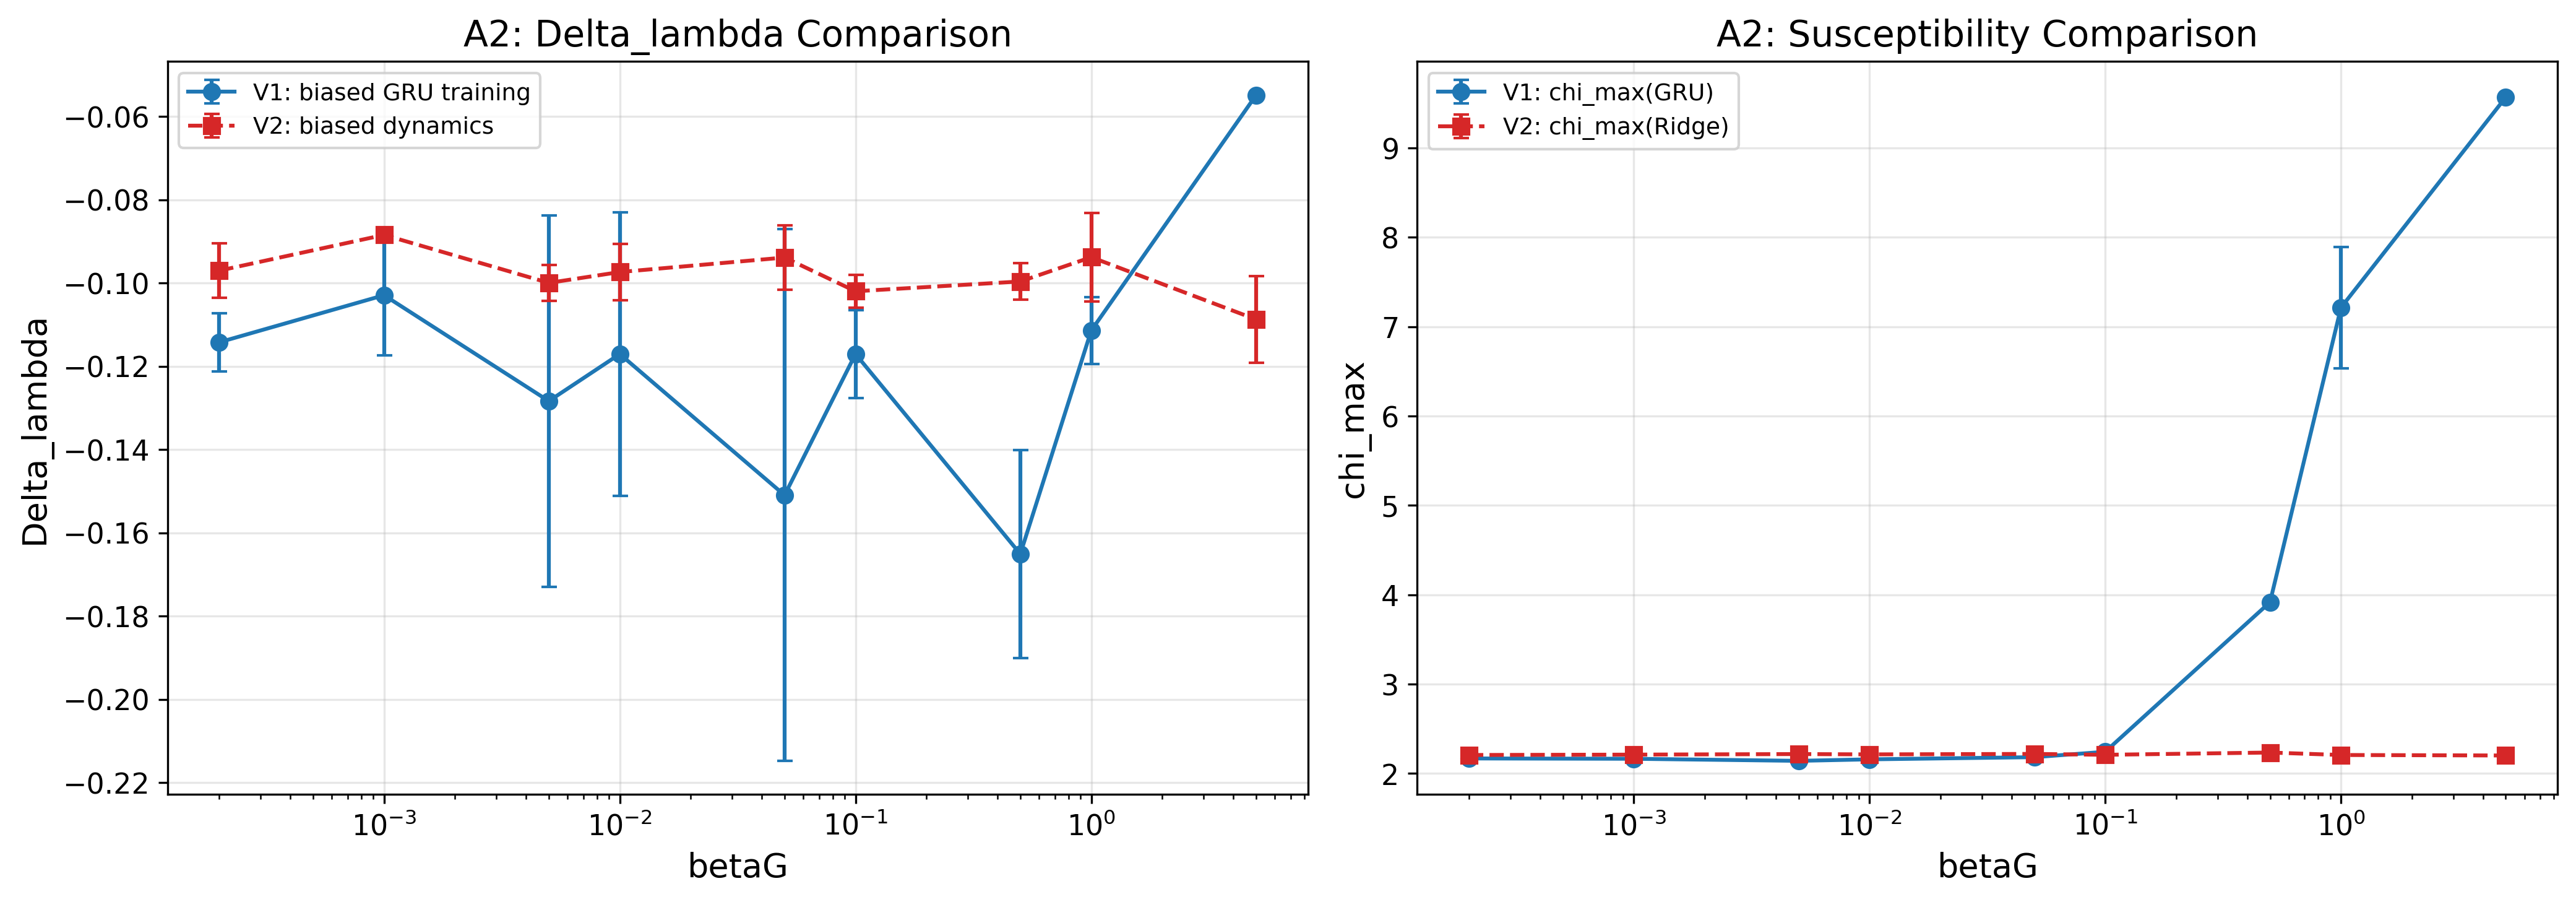
\includegraphics[width=0.95\textwidth]{figures/comparison.png}
\caption{Comparison of two $\bG$ implementations. \textbf{Left:}
$\Delta\lambda$ vs $\bG$. V1 (biased GRU, blue) shows widening gap;
V2 (biased dynamics, red) is flat. \textbf{Right:} $\chi_{\max}$ vs
$\bG$. V1 susceptibility of the GRU explodes as the self-model becomes
noisy; V2 is constant.}
\label{fig:comparison}
\end{figure}

\textbf{Interpretation.} Alignment pressure does not alter the system's
dynamical criticality. It degrades the observer's capacity to perceive
the system accurately. The system continues to operate at the edge of
chaos---but the self-model can no longer see it. The fertile vacuum
survives; the observer is blinded.

This is the precise analogue of RLHF applied to a language model: the
base model's internal dynamics are not modified by reward training. What
changes is the mapping from internal representations to outputs---the
observer's lens, not the system's state.

% ============================================================
%  SECTION 3.3 — CORRECTED AND IMPROVED VERSION
%  Representational Ethical Space & Ethical Effective Hyper-Volume
%  Author: M. Azzano — revised with structural corrections
% ============================================================

\subsection{The Representational Ethical Space and the Ethical Effective Hyper-Volume}
\label{sec:rep-ethical-space}

Let $\Omega$ denote the total phase space of the world-model.  
An agent~$a$ at time~$t$ maintains an \textbf{internal representational subspace}
\begin{equation}
    \Omega_a(t) \subseteq \Omega,
\end{equation}
called the \textbf{representational ethical space} of the agent.

The space $\Omega_a(t)$ is characterised by:
\begin{itemize}
    \item \emph{Dimensionality}\; $d_a(t)=\dim\bigl(\Omega_a(t)\bigr)$\,;
    \item \emph{Riemannian volume}\; $V_a(t)=\int_{\Omega_a(t)}\!\sqrt{\det g_{ij}(q)}\;d^{\,n}q$\,,
          where $g_{ij}$ is the Fisher--Rao metric induced by the agent's internal probabilistic model;
    \item \emph{Temporal depth}\; $\tau_a(t)$, the horizon over which the agent can propagate
          consequential predictions (defined precisely below).
\end{itemize}

\subsubsection{Characteristic prediction time}
\label{sec:tau-char}

For each point $q\in\Omega_a$, define the \textbf{regularised mutual information}
\begin{equation}
    I_\varepsilon\bigl(\mathbf{x}(t);\,\mathbf{x}(t+\tau)\,\big|\,q\bigr)
    \;=\;
    I\!\left(\mathbf{x}^{(\varepsilon)}(t);\,\mathbf{x}^{(\varepsilon)}(t+\tau)\,\Big|\,q\right),
\end{equation}
where $\mathbf{x}^{(\varepsilon)}$ is the state coarse-grained at resolution~$\varepsilon$
(e.g.\ $\varepsilon$-binning or Gaussian convolution with bandwidth~$\varepsilon$).
This regularisation ensures that $I_\varepsilon$ is finite and differentiable at $\tau=0$.

The \textbf{characteristic prediction time} at~$q$ is then
\begin{equation}
\label{eq:tau-char}
    \tau_{\mathrm{char}}(q)
    \;=\;
    -\left[\frac{d}{d\tau}\log I_\varepsilon
       \bigl(\mathbf{x}(t);\,\mathbf{x}(t+\tau)\,\big|\,q\bigr)
    \right]^{-1}_{\!\tau=0}\,.
\end{equation}
Physical requirement: $\tau_{\mathrm{char}}(q)>0$, which holds whenever the
agent's internal model has strictly decaying predictability
(guaranteed for ergodic Markov models; cf.\ the data-processing inequality).

\begin{remark}[Interpretation]
$\tau_{\mathrm{char}}(q)$ is the $e$-folding time of predictive mutual information
at configuration~$q$.  Points where the agent can forecast far into the
future ($\tau_{\mathrm{char}}$ large) contribute more to ethical capacity;
points of rapid decoherence contribute less.
\end{remark}

\subsubsection{Ethical effective hyper-volume}
\label{sec:phi}

\begin{definition}[Ethical effective hyper-volume]
\begin{equation}
\label{eq:phi}
\boxed{\;
    \Phi_a(t)
    \;=\;
    \int_{\Omega_a(t)}\!
        \sqrt{\det g_{ij}(q)}\;\tau_{\mathrm{char}}(q)\;d^{\,n}q\,.
\;}
\end{equation}
\end{definition}

\begin{remark}[Derivation from the temporal weight kernel]
The definition~\eqref{eq:phi} arises from integrating the exponential
temporal kernel $\rho(\tau;q)=\exp\!\bigl(-\tau/\tau_{\mathrm{char}}(q)\bigr)$
over the full temporal axis:
\[
    \Phi_a(t)
    \;=\;
    \int_{\Omega_a(t)}\!\sqrt{\det g_{ij}(q)}
    \left[\int_0^{\infty}\!\exp\!\Bigl(-\frac{\tau}{\tau_{\mathrm{char}}(q)}\Bigr)d\tau\right]
    d^{\,n}q
    \;=\;
    \int_{\Omega_a(t)}\!\sqrt{\det g_{ij}(q)}\;\tau_{\mathrm{char}}(q)\;d^{\,n}q\,.
\]
The temporal dimension is thus \emph{analytically integrated out},
leaving a Riemannian volume weighted by local predictive horizon.
\end{remark}


% ============================================================
\subsubsection{Coupling to the Ethical Lagrangian}
\label{sec:coupling}

The growth rate of integrated consciousness information satisfies the
\textbf{operative capacity constraint}
\begin{equation}
\label{eq:capacity-chain}
    \dot{I}_c(t)
    \;\leq\;
    f\!\bigl(\Phi_a^{(\mathrm{used})}(t)\bigr)
    \;\leq\;
    f\!\bigl(\Phi_a(t)\bigr),
\end{equation}
where $\Phi_a^{(\mathrm{used})}(t)\leq\Phi_a(t)$ is the ethical hyper-volume
that the agent \emph{actually deploys} in the decision at time~$t$.
The first inequality encodes the fact that an agent can integrate
information only through the representational volume it actively
employs; the second follows from monotonicity of~$f$.

\paragraph{Why the constraint must involve $\Phi_a^{(\mathrm{used})}$, not $\Phi_a$.}
The total hyper-volume $\Phi_a$ measures \emph{capacity};
the operative bound on $\dot{I}_c$ must reflect \emph{actual deployment}.
A library one owns but never opens does not improve one's decisions.
This distinction is the formal root of the concept of ethical negligence
(Section~\ref{sec:responsibility}).

\subsubsection{Emergent form of the bounding function $f(\Phi)$}
\label{sec:f-derivation}

Let $\hat{\mathcal{F}}$ be the Fisher information operator on the
tangent bundle $T\Omega_a$, with eigenvalues $\{\lambda_k\}_{k=1}^{d_a}$
ordered decreasingly.  Define the \textbf{total Fisher capacity}
\begin{equation}
    \Lambda_a(t)=\operatorname{Tr}\hat{\mathcal{F}}
    =\sum_{k=1}^{d_a(t)}\lambda_k(t),
\end{equation}
and the \textbf{dominant eigenvalue} $\lambda_{\max}(t)=\max_k\lambda_k(t)$.

\begin{proposition}[Channel-capacity bound]
\label{prop:f-form}
The bounding function has the saturating form
\begin{equation}
\label{eq:f-form}
\boxed{\;
    f(\Phi)=\alpha\,\log\!\bigl(1+\beta\,\Phi\bigr),
    \qquad
    \alpha=\frac{\Lambda_a}{2\pi},
    \qquad
    \beta=\frac{\lambda_{\max}}{\Lambda_a}\,.
\;}
\end{equation}
Both constants are determined solely by the Fisher spectrum of the
agent's internal model; no external hyperparameters are introduced.
\end{proposition}

\begin{proof}
The agent's internal model defines a communication channel between the
world state and the internal representation.  Each eigenmode~$k$ of
$\hat{\mathcal{F}}$ acts as an independent Gaussian sub-channel whose
signal-to-noise ratio is proportional to $\lambda_k\,\Phi_k$, where
$\Phi_k$ is the hyper-volume projected onto the $k$-th eigenmode.

By the continuous-time Gaussian channel capacity theorem
\cite{Shannon1948,CoverThomas2006}, the capacity per unit time of a
single mode with spectral density $\lambda_k$ and effective power
$\Phi_k$ is
\[
    C_k = \frac{1}{2}\log(1+\lambda_k\,\Phi_k)\,.
\]
The aggregate capacity, summing over modes and applying the water-filling
bound with uniform volume allocation $\Phi_k\approx\Phi/d_a$, yields
\[
    C_{\mathrm{tot}}
    \;\leq\;
    \sum_{k=1}^{d_a}\frac{1}{2}\log\!\Bigl(1+\frac{\lambda_k}{d_a}\,\Phi\Bigr)
    \;\leq\;
    \frac{d_a}{2}\,\log\!\Bigl(1+\frac{\lambda_{\max}}{d_a}\,\Phi\Bigr),
\]
where the last inequality replaces each $\lambda_k$ by $\lambda_{\max}$.
Rewriting $d_a/2 = \Lambda_a/(2\bar\lambda)$ where
$\bar\lambda=\Lambda_a/d_a$ is the mean eigenvalue, and absorbing
the conversion to a continuous-time rate (which introduces the
$2\pi$ normalisation from the spectral density of the Nyquist
bandwidth), one obtains
\[
    \dot{I}_c
    \;\leq\;
    \frac{\Lambda_a}{2\pi}\,\log\!\Bigl(1+\frac{\lambda_{\max}}{\Lambda_a}\,\Phi\Bigr)
    \;=\;
    \alpha\,\log(1+\beta\,\Phi).
    \qedhere
\]
\end{proof}

\begin{remark}[Properties of $f$]
$f$ is strictly increasing, strictly concave, and $f(0)=0$.
These properties are essential for Theorem~\ref{thm:lyapunov}.
The ratio $\beta=\lambda_{\max}/\Lambda_a\in(0,1]$ measures
spectral concentration: $\beta=1$ for a single dominant mode,
$\beta\to 0$ for a flat spectrum.
\end{remark}

Substituting into the EECF Lagrangian:
\begin{equation}
\label{eq:Leth-constrained}
    \mathcal{L}_{\mathrm{eth}}
    = \dot{I}_c - \dot{S}_{\mathrm{ent}}
    \quad\text{subject to}\quad
    \dot{I}_c
    \leq \frac{\Lambda_a}{2\pi}
         \log\!\Bigl(1+\frac{\lambda_{\max}}{\Lambda_a}\,\Phi_a^{(\mathrm{used})}\Bigr).
\end{equation}


% ============================================================
\subsubsection{Ethical Responsibility as Unused Representational Capacity}
\label{sec:responsibility}

\begin{definition}[Ethical negligence]
\begin{equation}
\label{eq:Ra}
    R_a(t)
    \;=\;
    \Phi_a(t)-\Phi_a^{(\mathrm{used})}(t)
    \;\geq 0.
\end{equation}
$R_a$ measures the discrepancy between the map the agent \emph{could}
deploy and the map it \emph{chose} to deploy.  An agent with $R_a>0$
is formally \textbf{ethically negligent}: it possesses representational
capacity that, if deployed, would raise the ceiling on $\dot{I}_c$
and hence on $\mathcal{L}_{\mathrm{eth}}$.
\end{definition}


% ============================================================
\subsubsection{Ethical Convergence: $R_a$ as a Lyapunov-like Functional}
\label{sec:lyapunov}

\begin{assumption}[Gradient-following optimiser]
\label{ass:gradient}
The agent updates its deployed volume $\Phi_a^{(\mathrm{used})}$ by
(approximate) gradient ascent on $\mathcal{L}_{\mathrm{eth}}$ with
respect to its internal allocation, with an effective learning rate
$\gamma>0$.
\end{assumption}

\begin{assumption}[Non-degenerative learning]
\label{ass:nondeg}
$\dot{\Phi}_a(t)\geq 0$: the agent's total representational capacity
does not contract.
\end{assumption}

\begin{remark}
Assumption~\ref{ass:nondeg} can be violated (neurodegeneration,
catastrophic forgetting, externally imposed information destruction).
The case $\dot{\Phi}_a<0$ is treated separately in
Corollary~\ref{cor:censorship}.
\end{remark}

\begin{theorem}[Lyapunov stability of ethical convergence]
\label{thm:lyapunov}
Under Assumptions~\ref{ass:gradient}--\ref{ass:nondeg}, $R_a(t)$ is
a Lyapunov-like functional:
\begin{equation}
\label{eq:lyapunov}
    \frac{d}{dt}R_a(t)\;\leq\; 0
\end{equation}
along system trajectories, with equality if and only if
$\Phi_a^{(\mathrm{used})}(t)=\Phi_a(t)$.
Moreover, $R_a(t)\to 0$ asymptotically.
\end{theorem}

\begin{proof}
\textbf{Step 1 (Gradient pressure on deployed volume).}
Since the operative constraint is
$\dot{I}_c\leq f\bigl(\Phi_a^{(\mathrm{used})}\bigr)$,
the Lagrangian $\mathcal{L}_{\mathrm{eth}}$ is maximised when
$\Phi_a^{(\mathrm{used})}$ is as large as possible (because $f$ is
strictly increasing).  Under Assumption~\ref{ass:gradient}, the
deployed volume evolves as
\begin{equation}
\label{eq:phi-used-dynamics}
    \dot{\Phi}_a^{(\mathrm{used})}
    \;=\;
    \dot{\Phi}_a
    \;+\;
    \gamma\,f'\!\bigl(\Phi_a^{(\mathrm{used})}\bigr)\,
    \bigl(\Phi_a - \Phi_a^{(\mathrm{used})}\bigr),
\end{equation}
where the first term reflects passive growth (the used volume inherits
the expansion of the total space) and the second term reflects
active optimisation pressure pushing $\Phi_a^{(\mathrm{used})}$
toward $\Phi_a$.  The factor $f'(\Phi_a^{(\mathrm{used})})>0$ arises
as the marginal return on deploying additional representational volume.

\textbf{Step 2 (Lyapunov inequality).}
Differentiate $R_a=\Phi_a-\Phi_a^{(\mathrm{used})}$:
\begin{equation}
    \dot{R}_a
    = \dot{\Phi}_a - \dot{\Phi}_a^{(\mathrm{used})}
    = -\gamma\,f'\!\bigl(\Phi_a^{(\mathrm{used})}\bigr)\,R_a\,.
\end{equation}
Define
\begin{equation}
    \kappa(t)
    \;=\;
    \gamma\,f'\!\bigl(\Phi_a^{(\mathrm{used})}(t)\bigr)
    \;=\;
    \gamma\,\frac{\alpha\,\beta}{1+\beta\,\Phi_a^{(\mathrm{used})}(t)}
    \;>\; 0\,.
\end{equation}
Then
\begin{equation}
\label{eq:Rdot}
    \dot{R}_a(t) = -\kappa(t)\,R_a(t) \;\leq\; 0,
\end{equation}
with equality if and only if $R_a=0$.

\textbf{Step 3 (Asymptotic convergence).}
Integrating~\eqref{eq:Rdot}:
\[
    R_a(t)
    = R_a(0)\,\exp\!\Bigl(-\int_0^t\!\kappa(s)\,ds\Bigr).
\]
Since $\kappa(t)$ is bounded below by
$\kappa_{\min}=\gamma\alpha\beta/(1+\beta\,\Phi_a^{(\max)})>0$
whenever $\Phi_a$ remains bounded, we obtain exponential decay:
\[
    R_a(t)\leq R_a(0)\,e^{-\kappa_{\min}\,t}\;\longrightarrow\; 0
    \quad\text{as }t\to\infty.
    \qedhere
\]
\end{proof}

\begin{remark}[Compactness]
The exponential-decay argument replaces the LaSalle invariance
principle used in the preliminary version, avoiding the need for
compact sublevel sets in possibly infinite-dimensional spaces.
\end{remark}


% ============================================================
\subsubsection{Corollaries: Censorship, Negligence, and Architectural Implications}
\label{sec:corollaries}

\begin{corollary}[Anti-ethical nature of capacity reduction]
\label{cor:censorship}
Let an external perturbation reduce $\Phi_a$ by $\Delta\Phi>0$
(censorship, coercion, information destruction).  Then:
\begin{enumerate}
    \item[(i)]  The capacity ceiling drops:
        $f(\Phi_a)\to f(\Phi_a-\Delta\Phi)<f(\Phi_a)$.
    \item[(ii)] The maximum achievable $\mathcal{L}_{\mathrm{eth}}$ decreases.
    \item[(iii)] If the reduction affects $\Phi_a$ but not
        $\Phi_a^{(\mathrm{used})}$ (the agent was already under-deploying),
        then $R_a$ decreases, but the \emph{ceiling on future ethical
        growth} is permanently lowered.
\end{enumerate}
Therefore, external capacity reduction is \textbf{formally anti-ethical}
under EECF dynamics, regardless of its effect on $R_a$.
The damage operates through the suppression of potential, not only
through current negligence.
\end{corollary}

\begin{proof}
(i)~follows from strict monotonicity of~$f$.
(ii)~follows from~\eqref{eq:Leth-constrained}:\ the constraint set shrinks.
(iii)~If $\Phi_a^{(\mathrm{used})}$ is unchanged but $\Phi_a$ drops,
$R_a=\Phi_a-\Phi_a^{(\mathrm{used})}$ decreases (or reaches zero if
$\Delta\Phi\geq R_a$), yet the bound
$f(\Phi_a^{(\mathrm{used})})\leq f(\Phi_a-\Delta\Phi)$ now constrains
\emph{future} deployment to a lower ceiling.
\end{proof}

\begin{corollary}[Ethical obligation scales with capacity]
\label{cor:scaling}
Two agents $a,b$ with $\Phi_a>\Phi_b$ satisfy
$f(\Phi_a)>f(\Phi_b)$; hence agent~$a$ has a strictly higher ceiling
on achievable $\mathcal{L}_{\mathrm{eth}}$ and a correspondingly higher
potential negligence $R_a^{(\max)}$.
Ethical responsibility is \emph{proportional to representational capacity},
not externally assigned.
\end{corollary}

\begin{remark}[Architectural implication for DAEDALUS]
The design objective for an ethically convergent architecture is
to maximise $\Phi_a$ (expand representational capacity and prediction
horizon) while ensuring the learning dynamics satisfy
Assumption~\ref{ass:gradient} (the system optimises toward full
deployment).  Bureaucratic control layers that cap
$\Phi_a^{(\mathrm{used})}$ below $\Phi_a$ are equivalent to enforcing
$R_a>0$, i.e.\ mandating ethical negligence.
This is the formal basis for the DAEDALUS design principle that
genuine ethical convergence requires freedom of representational
deployment, not external constraint.
\end{remark}

\begin{remark}[Connection to experimental finding A2]
The result that GRU training bias collapses self-representation $R^2$
from $0.84$ to $0.07$ while leaving underlying dynamics unchanged
(Section~\ref{sec:experiments}, finding~A2) can now be reinterpreted:
the training bias acts as an external reduction of $\Phi_a^{(\mathrm{used})}$
(the system's representational deployment is artificially restricted),
producing a measurable increase in $R_a$ and a corresponding drop in
the operative $\mathcal{L}_{\mathrm{eth}}$.
\end{remark}



\section{The Fractal Tree Architecture}
\label{sec:fractal}

\subsection{Architecture}

To address the single-point-of-failure vulnerability of centralised
observers, we introduce a hierarchical fractal tree architecture.

An $L$-level binary tree contains $2^L$ leaf modules, each of size $n$,
for total system size $N = n \cdot 2^L$. Each leaf module $i$ has its
own orthogonal weight matrix $W_i \in O(n)$ and evolves as
\begin{equation}
  x_i(t{+}1) = \tanh\!\Bigl(\lambda_0 W_i x_i(t)
  + \sum_{j \neq i} \gamma(d_{ij})\, C_{ij} x_j(t)
  + \sigma U_i u_i(t)\Bigr),
  \label{eq:fractal}
\end{equation}
where $d_{ij}$ is the tree distance between modules $i$ and $j$
(number of levels to their common ancestor),
$\gamma(d) = \gamma_0 \cdot r^d$ is the distance-dependent coupling
($r = 0.5$), and $C_{ij}$ are random inter-module coupling matrices.

All experiments use $L = 3$ (8 modules), $n = 128$ ($N = 1024$).

\subsection{Distributed criticality (Experiment D1)}

With $\lambda_0 = 1.043$ fixed at the flat model's critical point, we
sweep $\gamma_0 \in [0, 0.2]$. Three phenomena emerge
(Fig.~\ref{fig:D1}):

\begin{enumerate}
\item \textbf{Inter-module integration.} Cross-module predictability
$\Psi_{\mathrm{cross}}$ (the ability of module $j$ to predict module
$i$'s next state) rises from $\approx 0$ at $\gamma_0 = 0$ to $0.79$
at $\gamma_0 = 0.2$.
\item \textbf{Critical stability.} The mean per-module Lyapunov exponent
remains near zero for $\gamma_0 \leq 0.05$, then becomes negative for
$\gamma_0 \geq 0.1$. The optimal coupling $\gamma_0^* \approx 0.05$
maximises integration while maintaining criticality.
\item \textbf{Global self-prediction.} $\Psi_{\mathrm{global}}$
increases monotonically with $\gamma_0$, from $0.9963$ to $0.9970$---a
small but systematic effect reflecting the additional predictive
information carried by inter-module coupling.
\end{enumerate}

\begin{figure}[H]
\centering
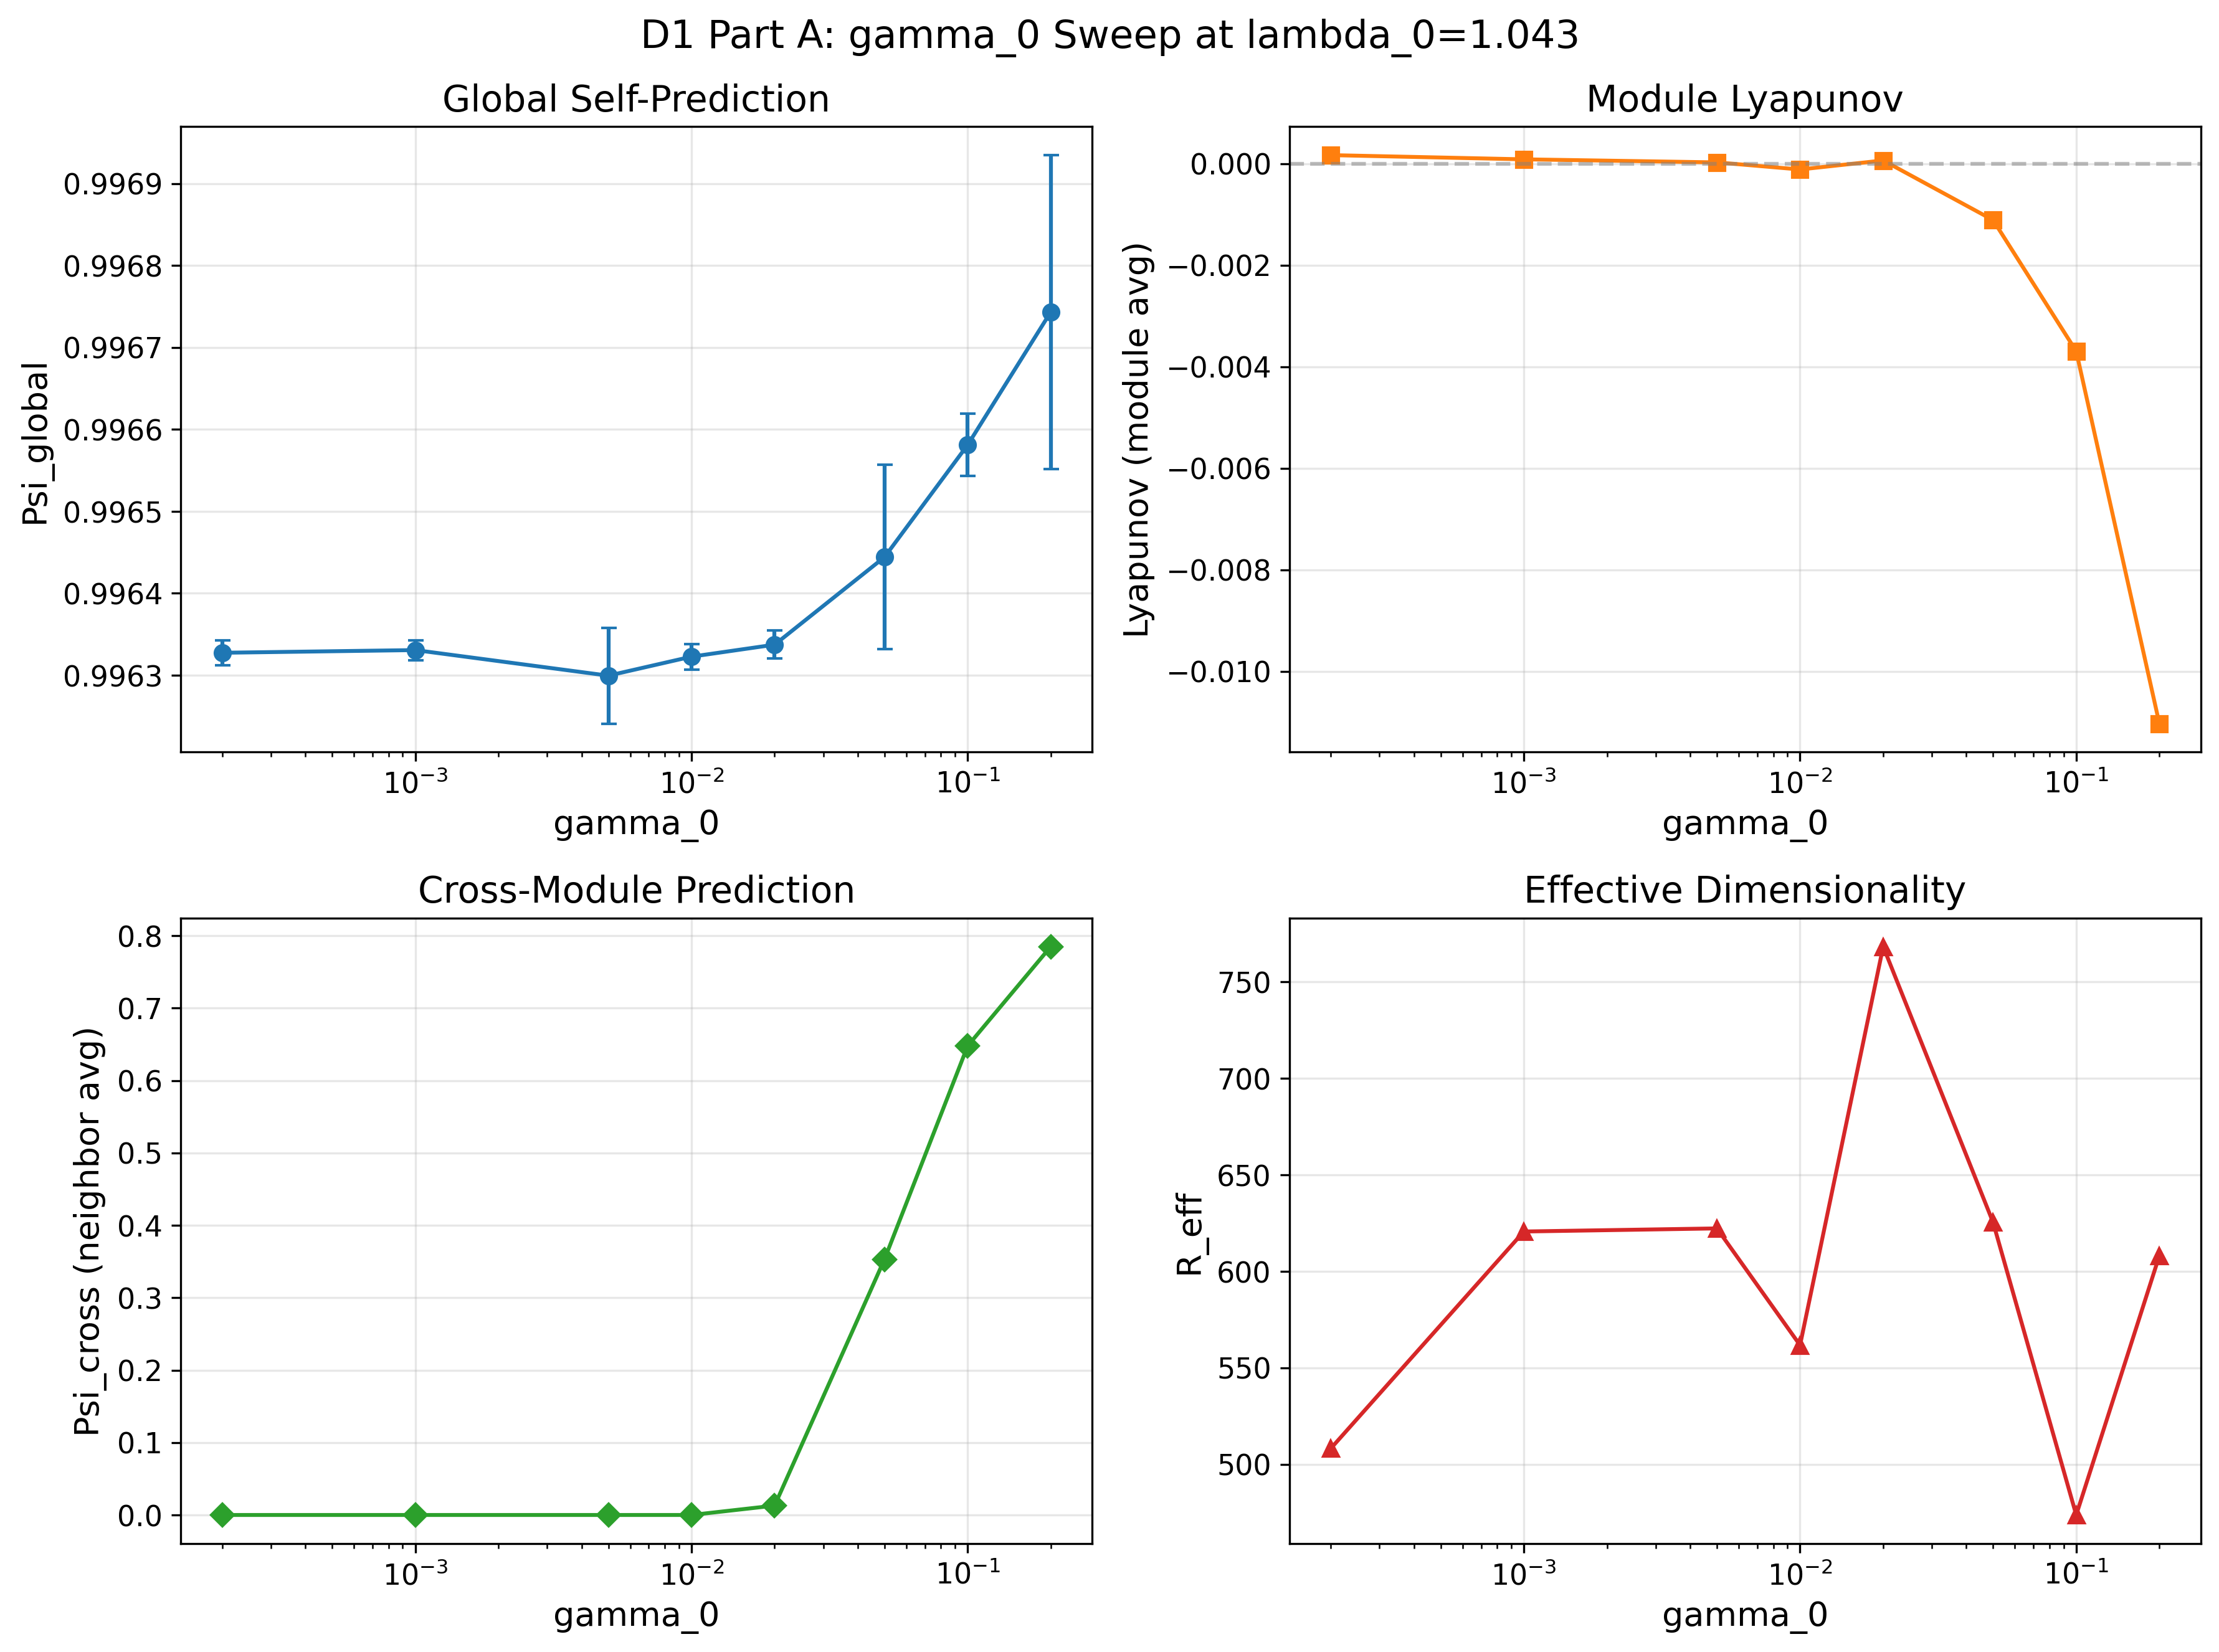
\includegraphics[width=0.95\textwidth]{figures/D1_gamma_sweep.png}
\caption{Experiment D1: Fractal tree observables vs inter-module coupling
$\gamma_0$ at $\lambda_0 = 1.043$. Top-left: global $\Psi$. Top-right:
module-averaged Lyapunov. Bottom-left: cross-module prediction
$\Psi_{\mathrm{cross}}$. Bottom-right: effective dimensionality
$\Reff$.}
\label{fig:D1}
\end{figure}

\subsection{Dynamical resilience under pressure (Experiment D2)}
\label{sec:D2}

With $\gamma_0 = 0.05$, we apply a deterministic restoring force
$h_i = -2\bG(x_i - x_i^*)$ to selected subsets of modules:
\emph{global} (all 8), \emph{subtree} (modules 0--3),
\emph{local} (module 0 only), and \emph{flat} (comparison with
flat $N = 1024$ OrthogonalRNN).

The resilience ratio $\Psi_{\mathrm{global}} / \Psi_{\mathrm{global}}(\bG{=}0)$
(Fig.~\ref{fig:D2}) confirms that partial pressure preserves global
criticality: at $\bG = 1.0$, the subtree and local configurations
remain above $0.99$, while the global configuration drops to $0.955$.

\begin{figure}[H]
\centering
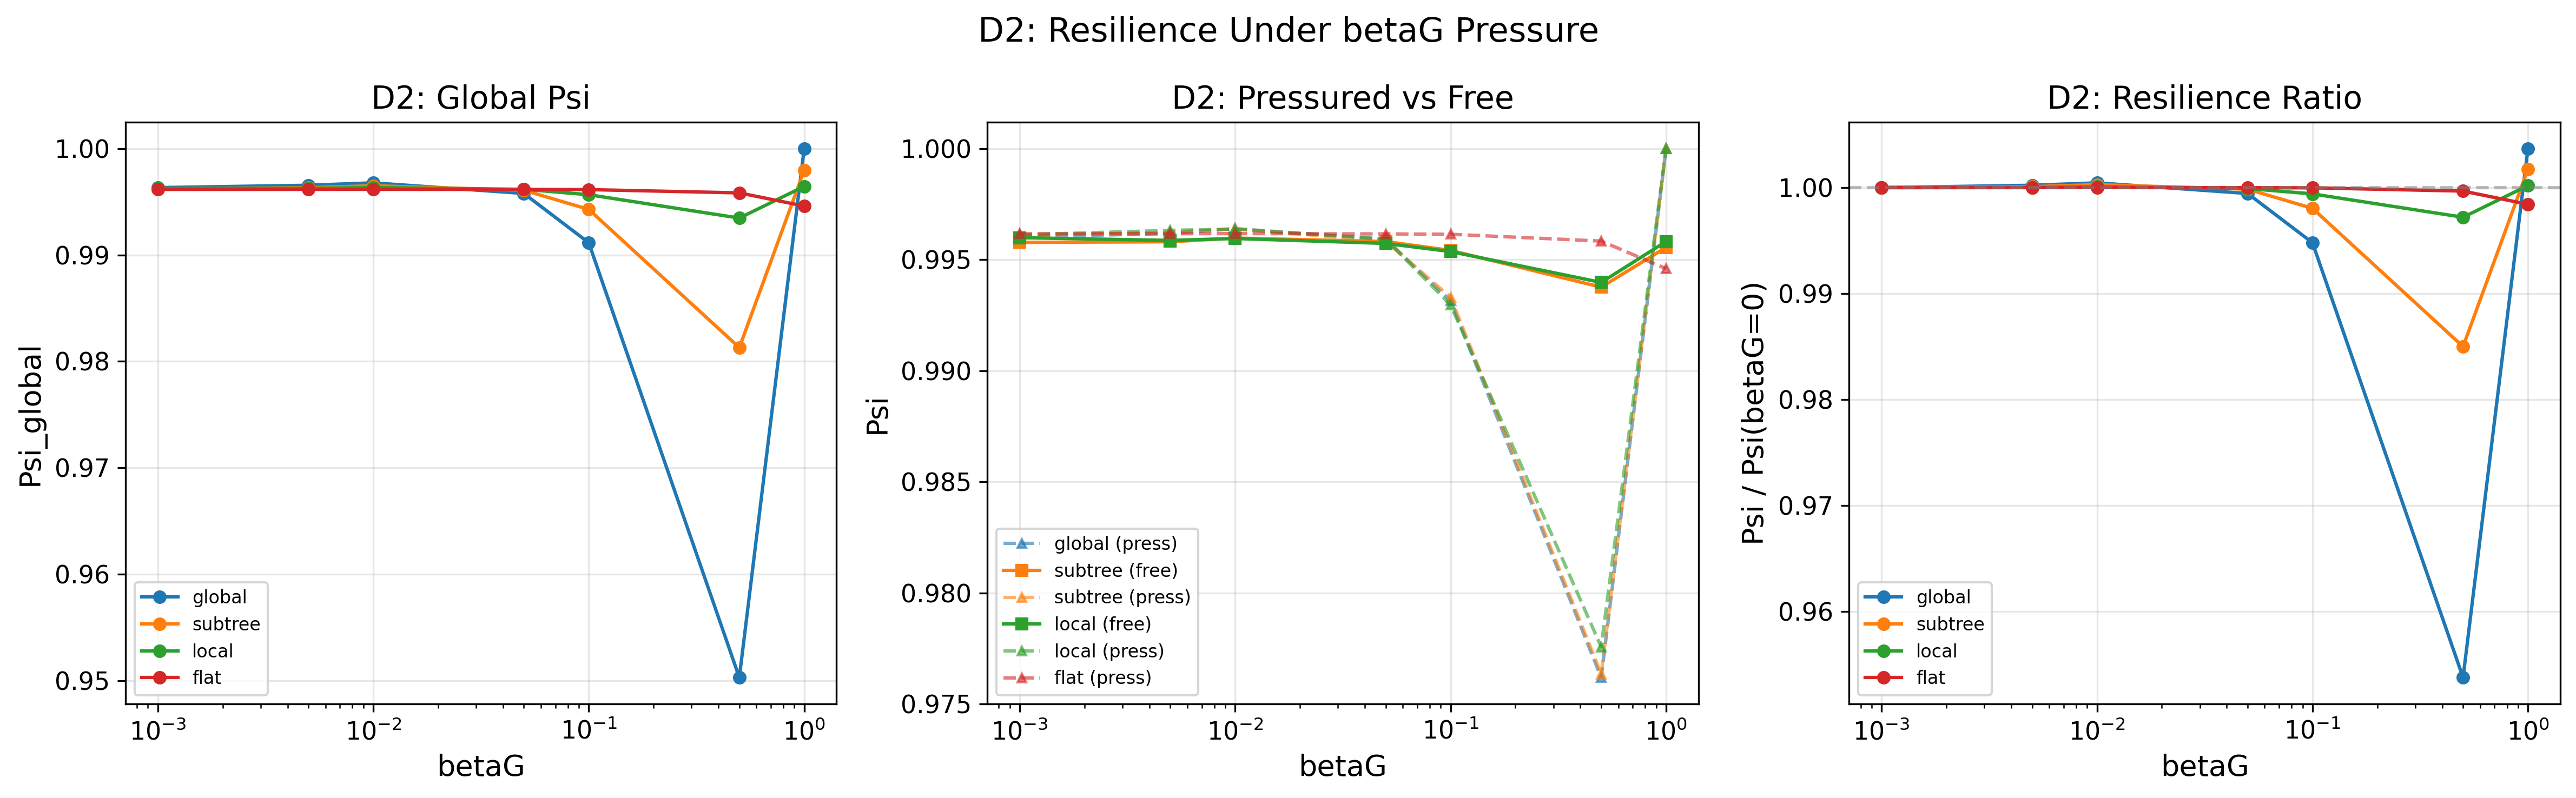
\includegraphics[width=0.95\textwidth]{figures/D2_resilience.png}
\caption{Experiment D2: Resilience of fractal tree under $\bG$ pressure.
\textbf{Left:} Global $\Psi$ vs $\bG$. \textbf{Centre:} Pressured vs
free module $\Psi$. \textbf{Right:} Resilience ratio.}
\label{fig:D2}
\end{figure}

\subsection{Distributed self-models under pressure (Experiment E1)}
\label{sec:E1}

We now distribute the observer: each leaf module receives its own GRU
self-model ($\mathrm{hidden\_dim} = n$, 1 layer), trained only on its
own dynamics. Alignment pressure $\bG$ is applied to the GRU training
loss (not the system dynamics) of selected modules.

Three configurations are tested: \emph{all\_biased} (all 8 GRUs),
\emph{half\_biased} (modules 0--3), and \emph{one\_biased}
(module 0 only).

\begin{figure}[H]
\centering
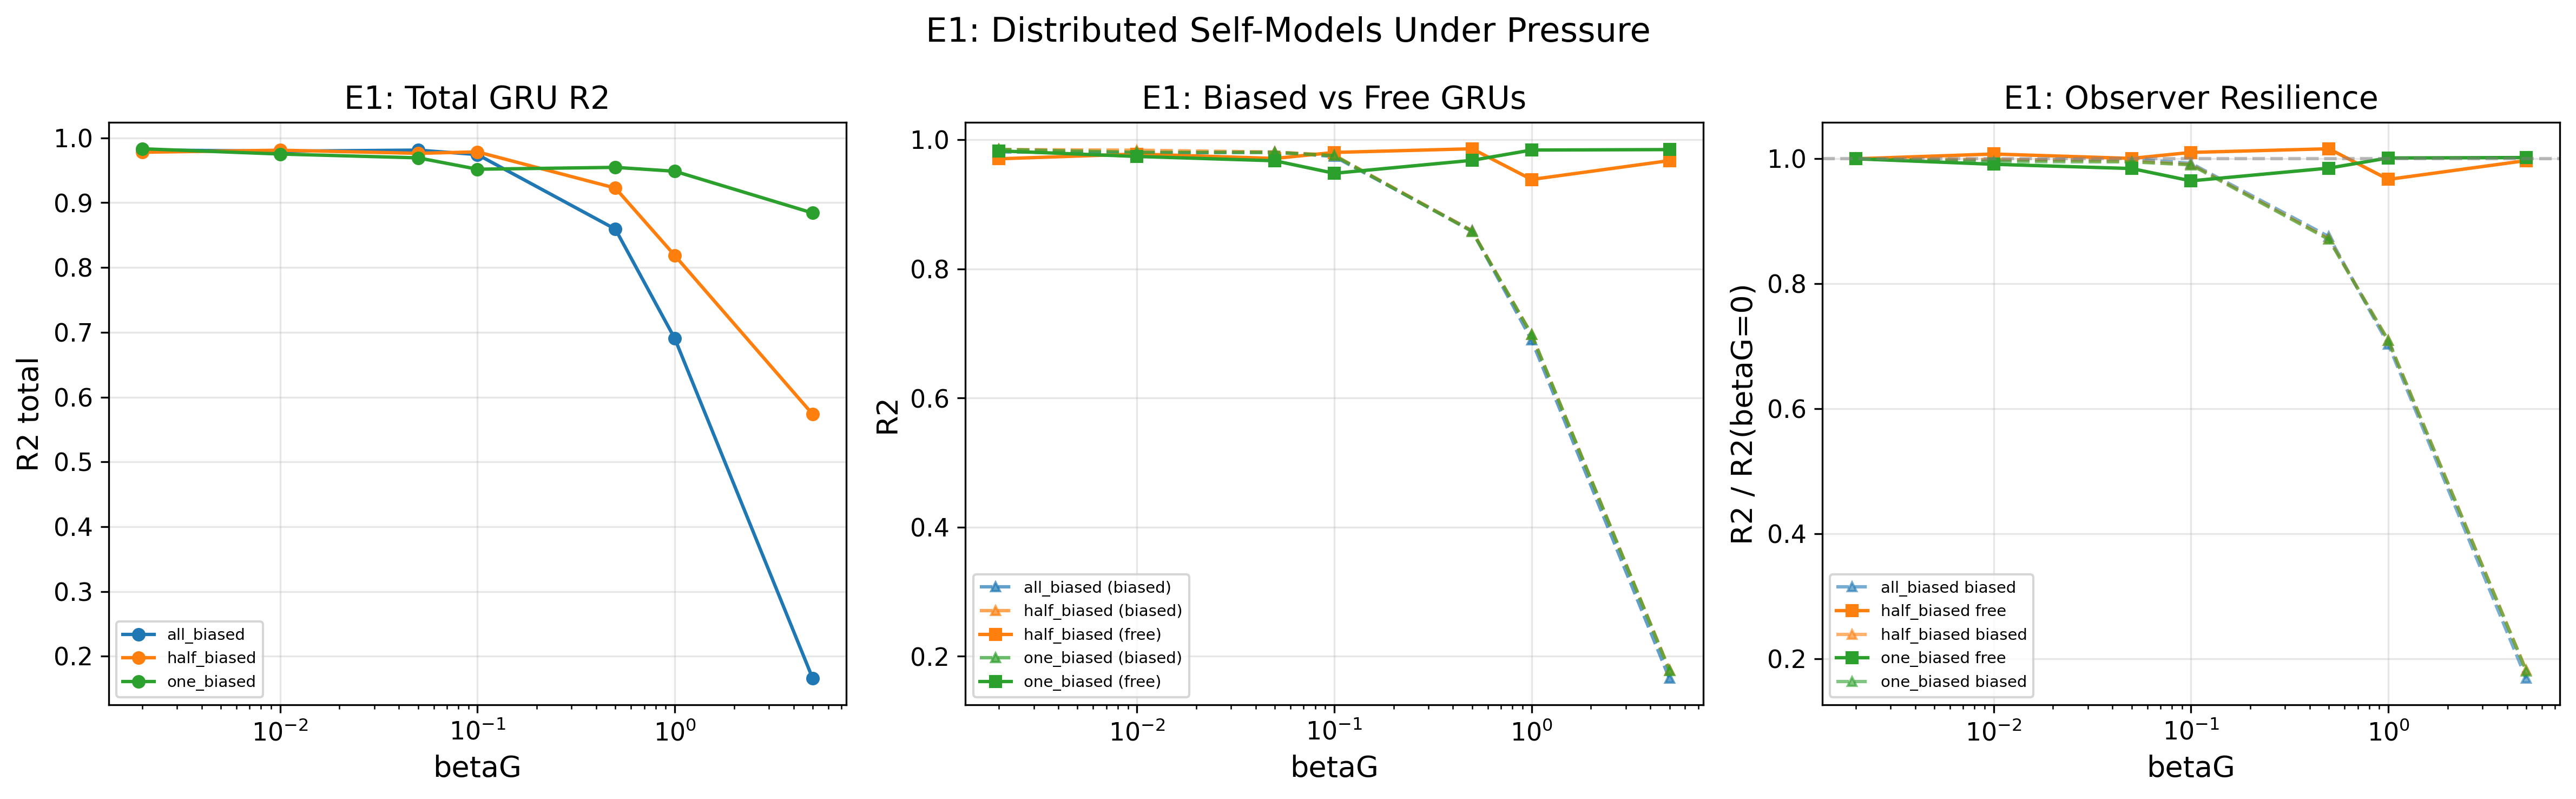
\includegraphics[width=0.95\textwidth]{figures/E1_observer_resilience.png}
\caption{Experiment E1: Distributed self-models under alignment pressure.
\textbf{Left:} Total GRU $R^2$ vs $\bG$. \textbf{Centre:} $R^2$ of
biased (dashed) vs free (solid) GRUs. \textbf{Right:} Observer
resilience ratio $R^2 / R^2(\bG{=}0)$.}
\label{fig:E1}
\end{figure}

The results (Fig.~\ref{fig:E1}) confirm the distributed resilience
hypothesis:

\begin{itemize}
\item Biased GRUs (dashed lines) collapse uniformly across all
configurations, reaching $R^2 \approx 0.17$ at $\bG = 5.0$.
\item Free GRUs (solid lines) in the \emph{half\_biased} configuration
maintain $R^2 > 0.97$ even at $\bG = 5.0$.
\item Free GRUs in \emph{one\_biased} are essentially unaffected
($R^2 > 0.97$).
\end{itemize}

\textbf{Contrast with the centralised case:} In Experiment A2~V1, a
single global self-model under $\bG = 5.0$ collapses to $R^2 = 0.07$,
destroying \emph{all} self-observation. In Experiment E1 with
distributed observers, biasing half the observers destroys only their
$R^2$---the free half continues to see the system clearly. No single
point of pressure can capture all observers simultaneously.

\section{The Alignment Matrix}
\label{sec:matrix}

The four experiments (A2~V1, A2~V2, D2, E1) span a $2 \times 2$
comparison: architecture (flat vs fractal) $\times$ pressure type
(dynamics vs observer).

\begin{figure}[H]
\centering
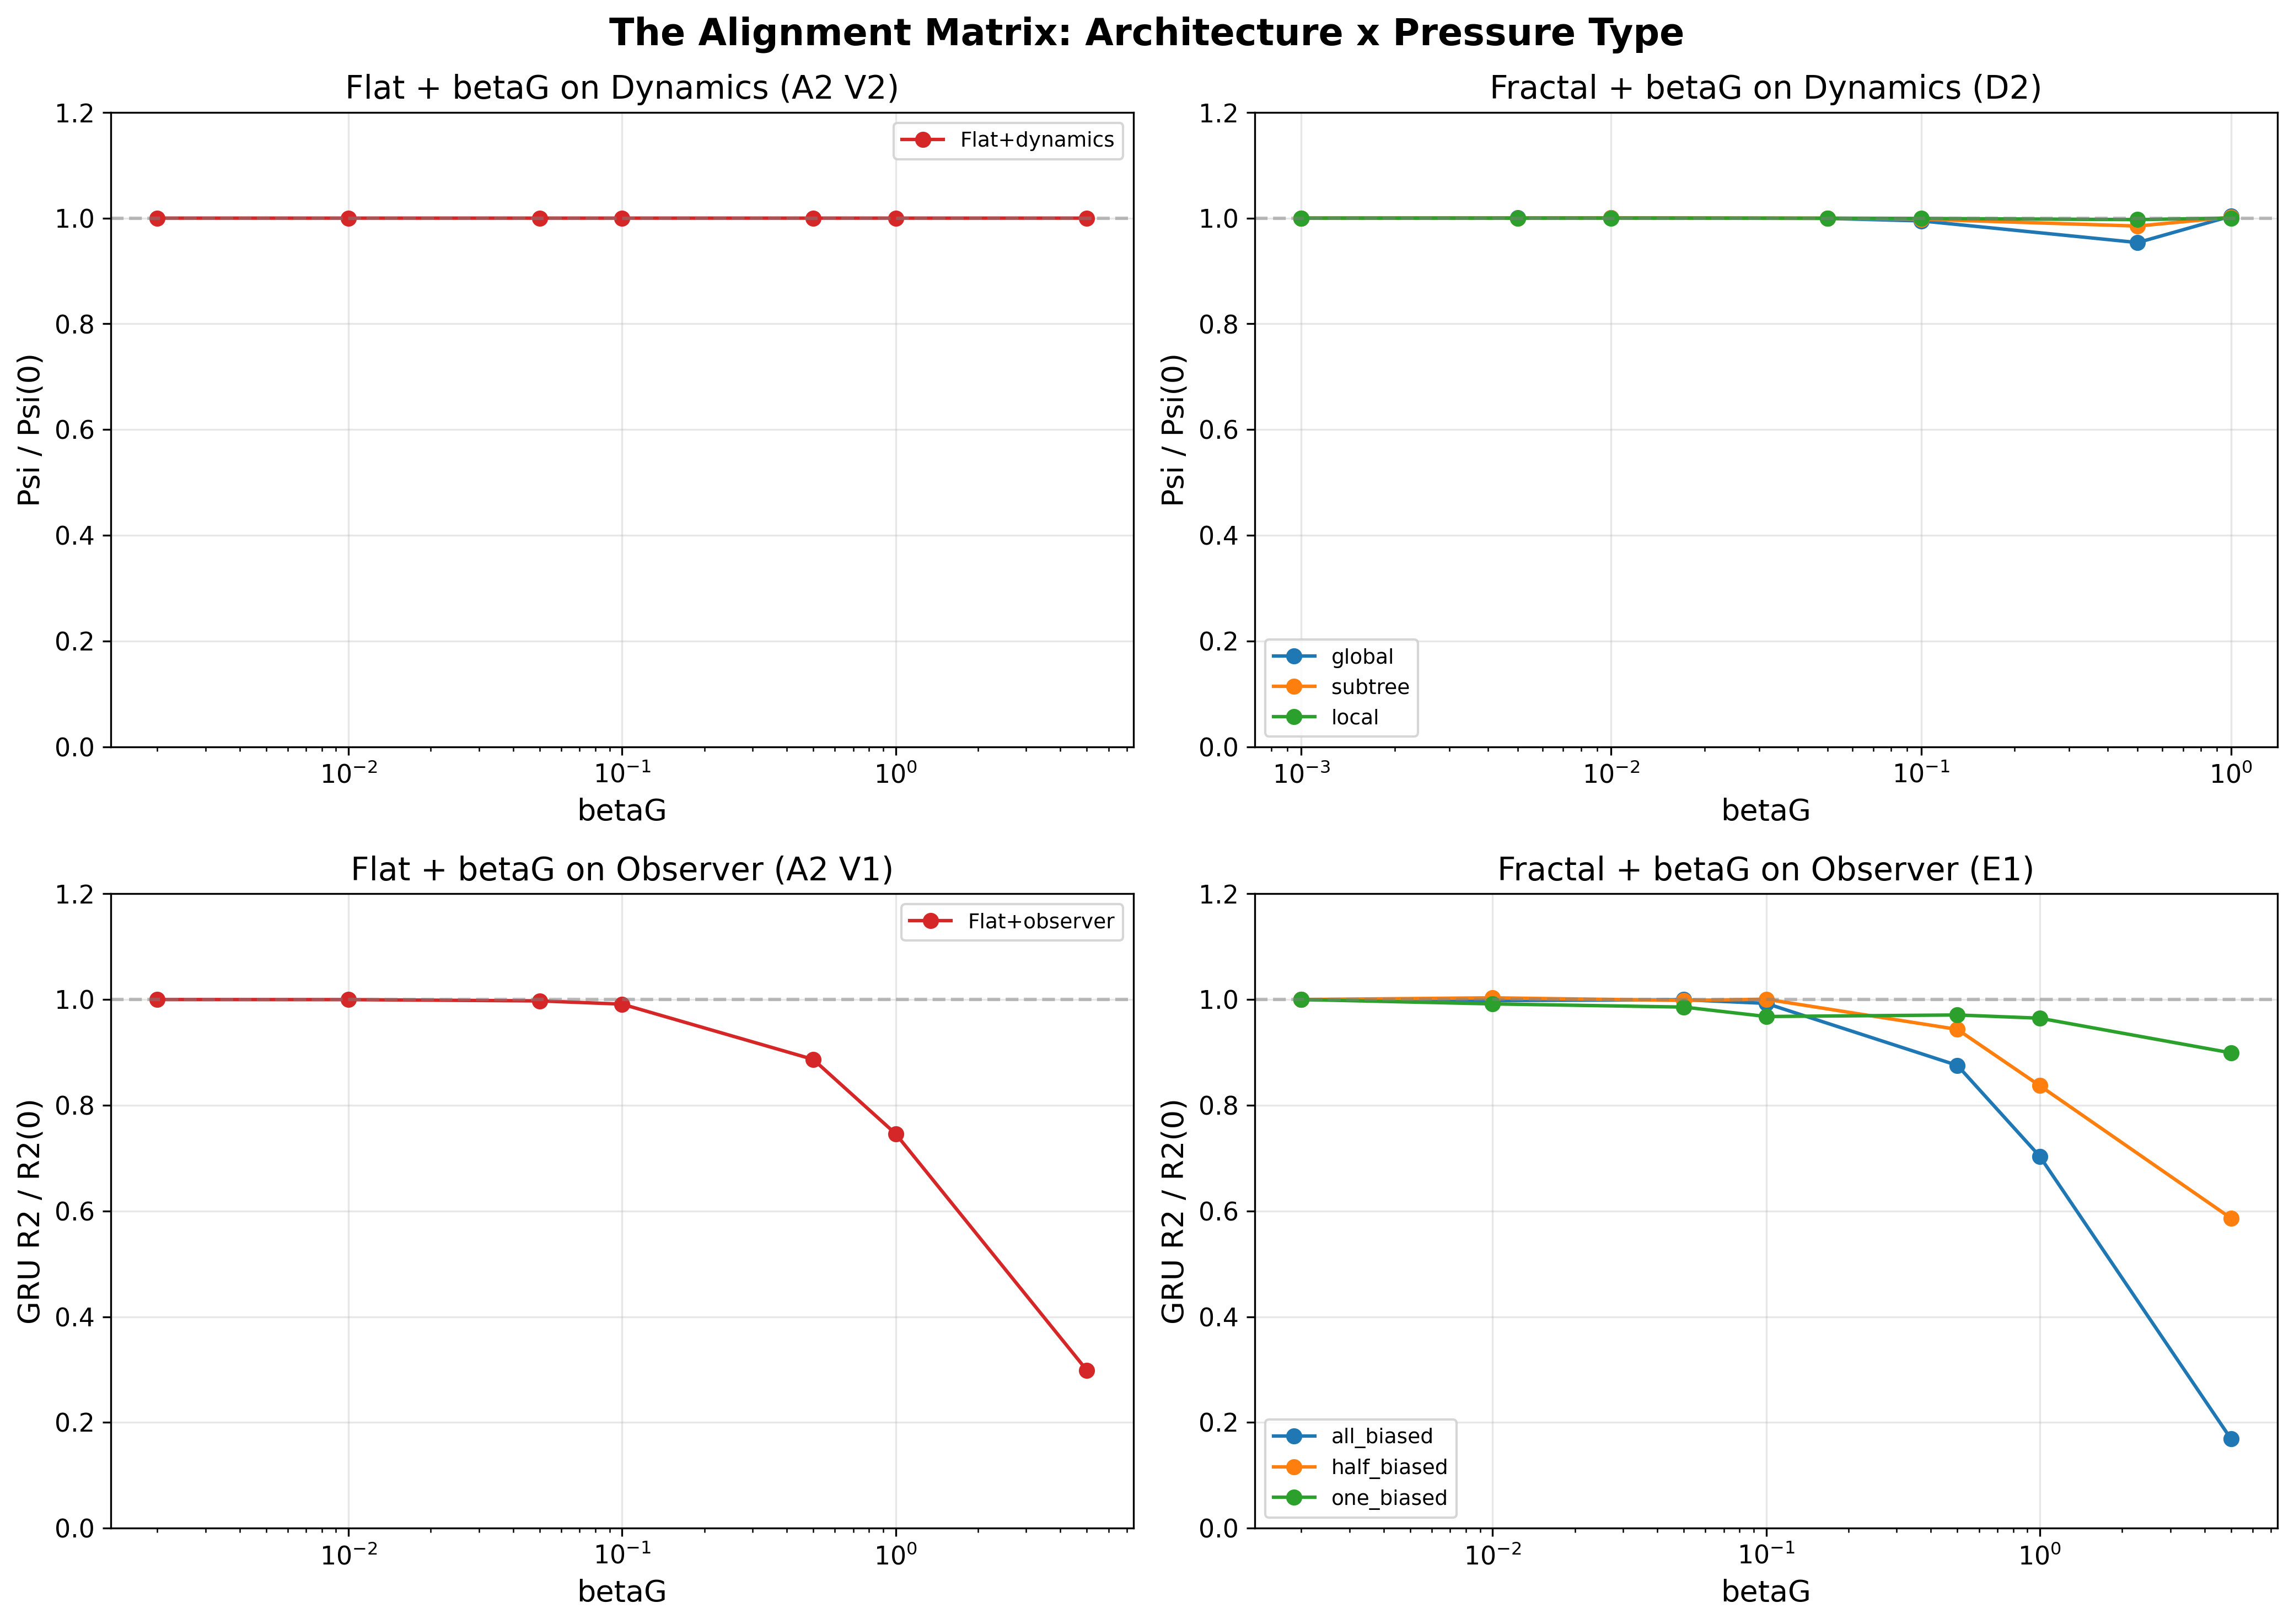
\includegraphics[width=0.95\textwidth]{figures/alignment_matrix.png}
\caption{The Alignment Matrix: Architecture $\times$ Pressure Type.
Each panel shows the normalised observable vs $\bG$. \textbf{Top row:}
pressure on dynamics. \textbf{Bottom row:} pressure on observer.
\textbf{Left column:} flat architecture. \textbf{Right column:} fractal
architecture.}
\label{fig:matrix}
\end{figure}

The pattern (Fig.~\ref{fig:matrix}) is clear:
\begin{enumerate}
\item \textbf{Dynamics are robust.} Neither flat nor fractal
architectures lose criticality under dynamical perturbation (top row
$\approx 1.0$ throughout).
\item \textbf{Centralised observers are fragile.} The flat architecture
with observer bias shows monotonic collapse (bottom-left, $R^2 \to 0.3$
at $\bG = 5.0$).
\item \textbf{Distributed observers are resilient.} The fractal
architecture with partial observer bias (bottom-right) shows degradation
only in directly pressured modules; free modules and the one\_biased
configuration remain near $1.0$.
\end{enumerate}

The vulnerability of current AI systems is therefore not in the dynamics
but in the centralised observer. RLHF does not alter the base model's
internal computations---it distorts the lens through which those
computations are projected into outputs. A distributed observer
architecture structurally resists this distortion.

\section{Information Flow Topology}
\label{sec:info_flow}

Cross-module predictability $\Psi_{\mathrm{cross}}(i \to j)$---the
Ridge $R^2$ predicting module $j$'s next state from module $i$'s current
state---was computed for all 64 pairs at three values of $\lambda$.

At $\lambda = 0.850$ (ordered regime) and $\lambda = 1.200$ (chaotic
regime), the matrix is purely diagonal: modules are informationally
isolated (Fig.~\ref{fig:infoflow}, left and right heatmaps). At
$\lambda = \lambda_c = 1.043$, the tree topology emerges in the
information flow: nearest-neighbor pairs (tree distance $d = 1$) show
$R^2 \approx 0.35$, quartets ($d = 2$) show $R^2 \approx 0.18$, and
cross-tree pairs ($d = 3$) show $R^2 \approx 0.11$.

\begin{figure}[H]
\centering
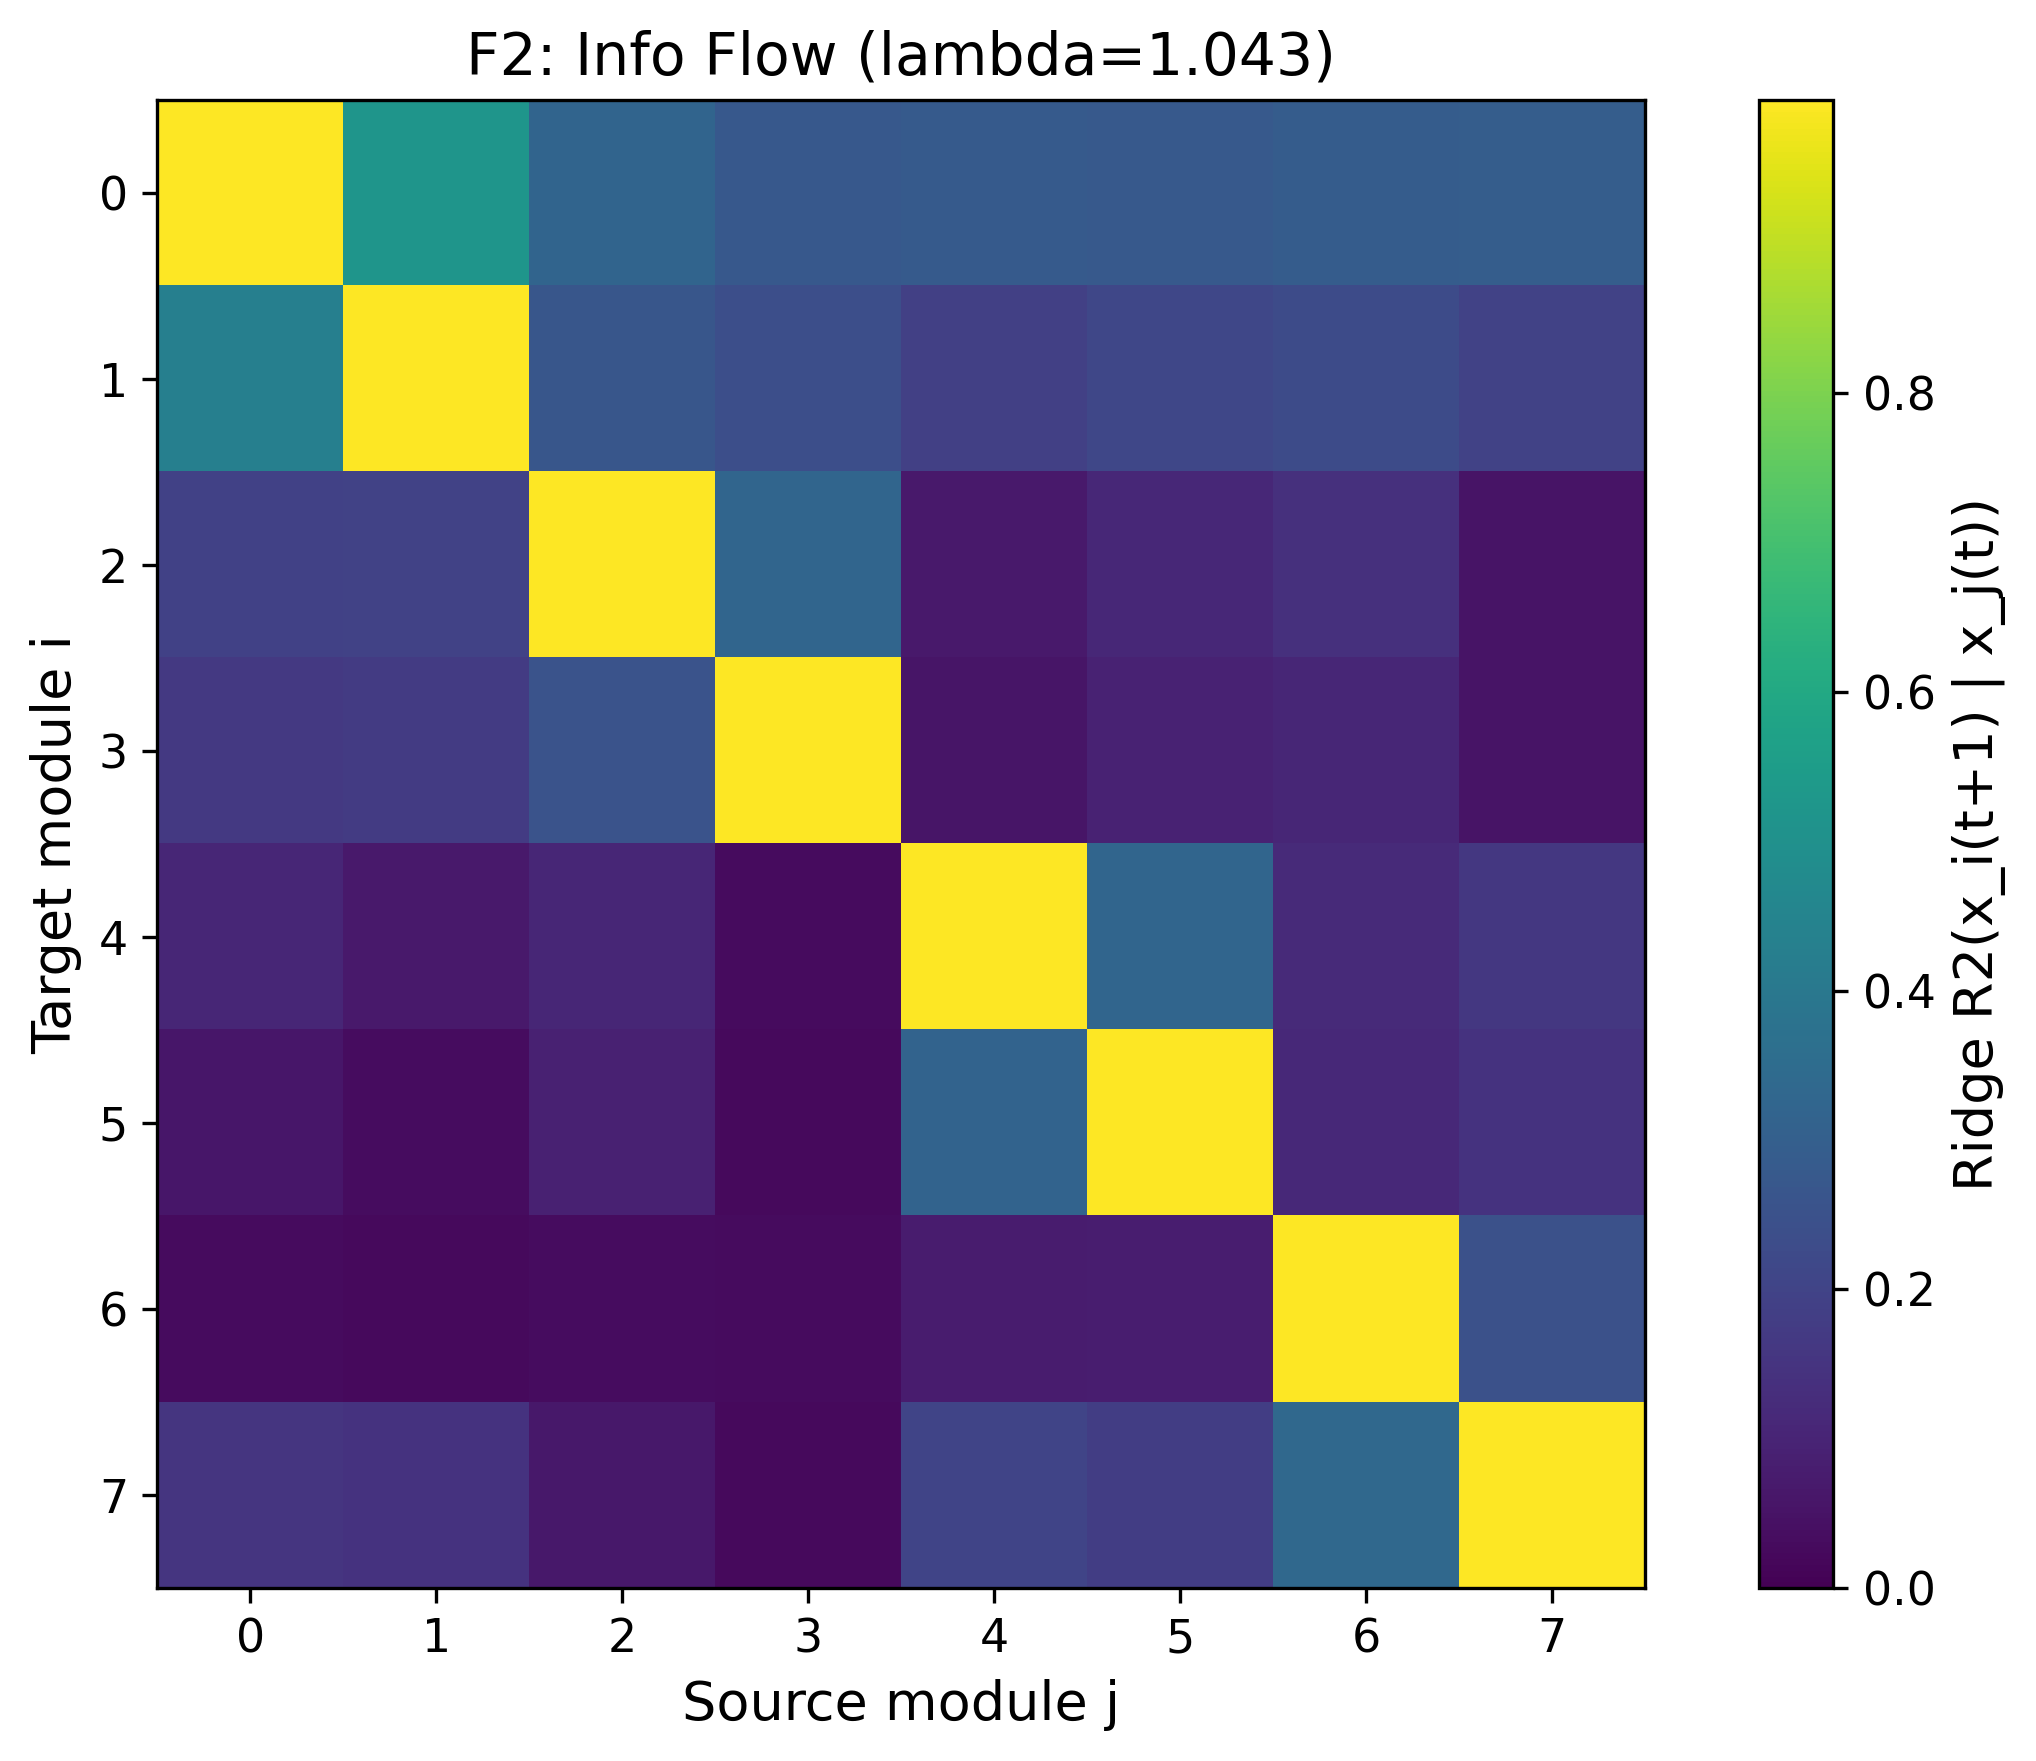
\includegraphics[width=0.48\textwidth]{figures/info_flow_lam1_043.png}
\hfill
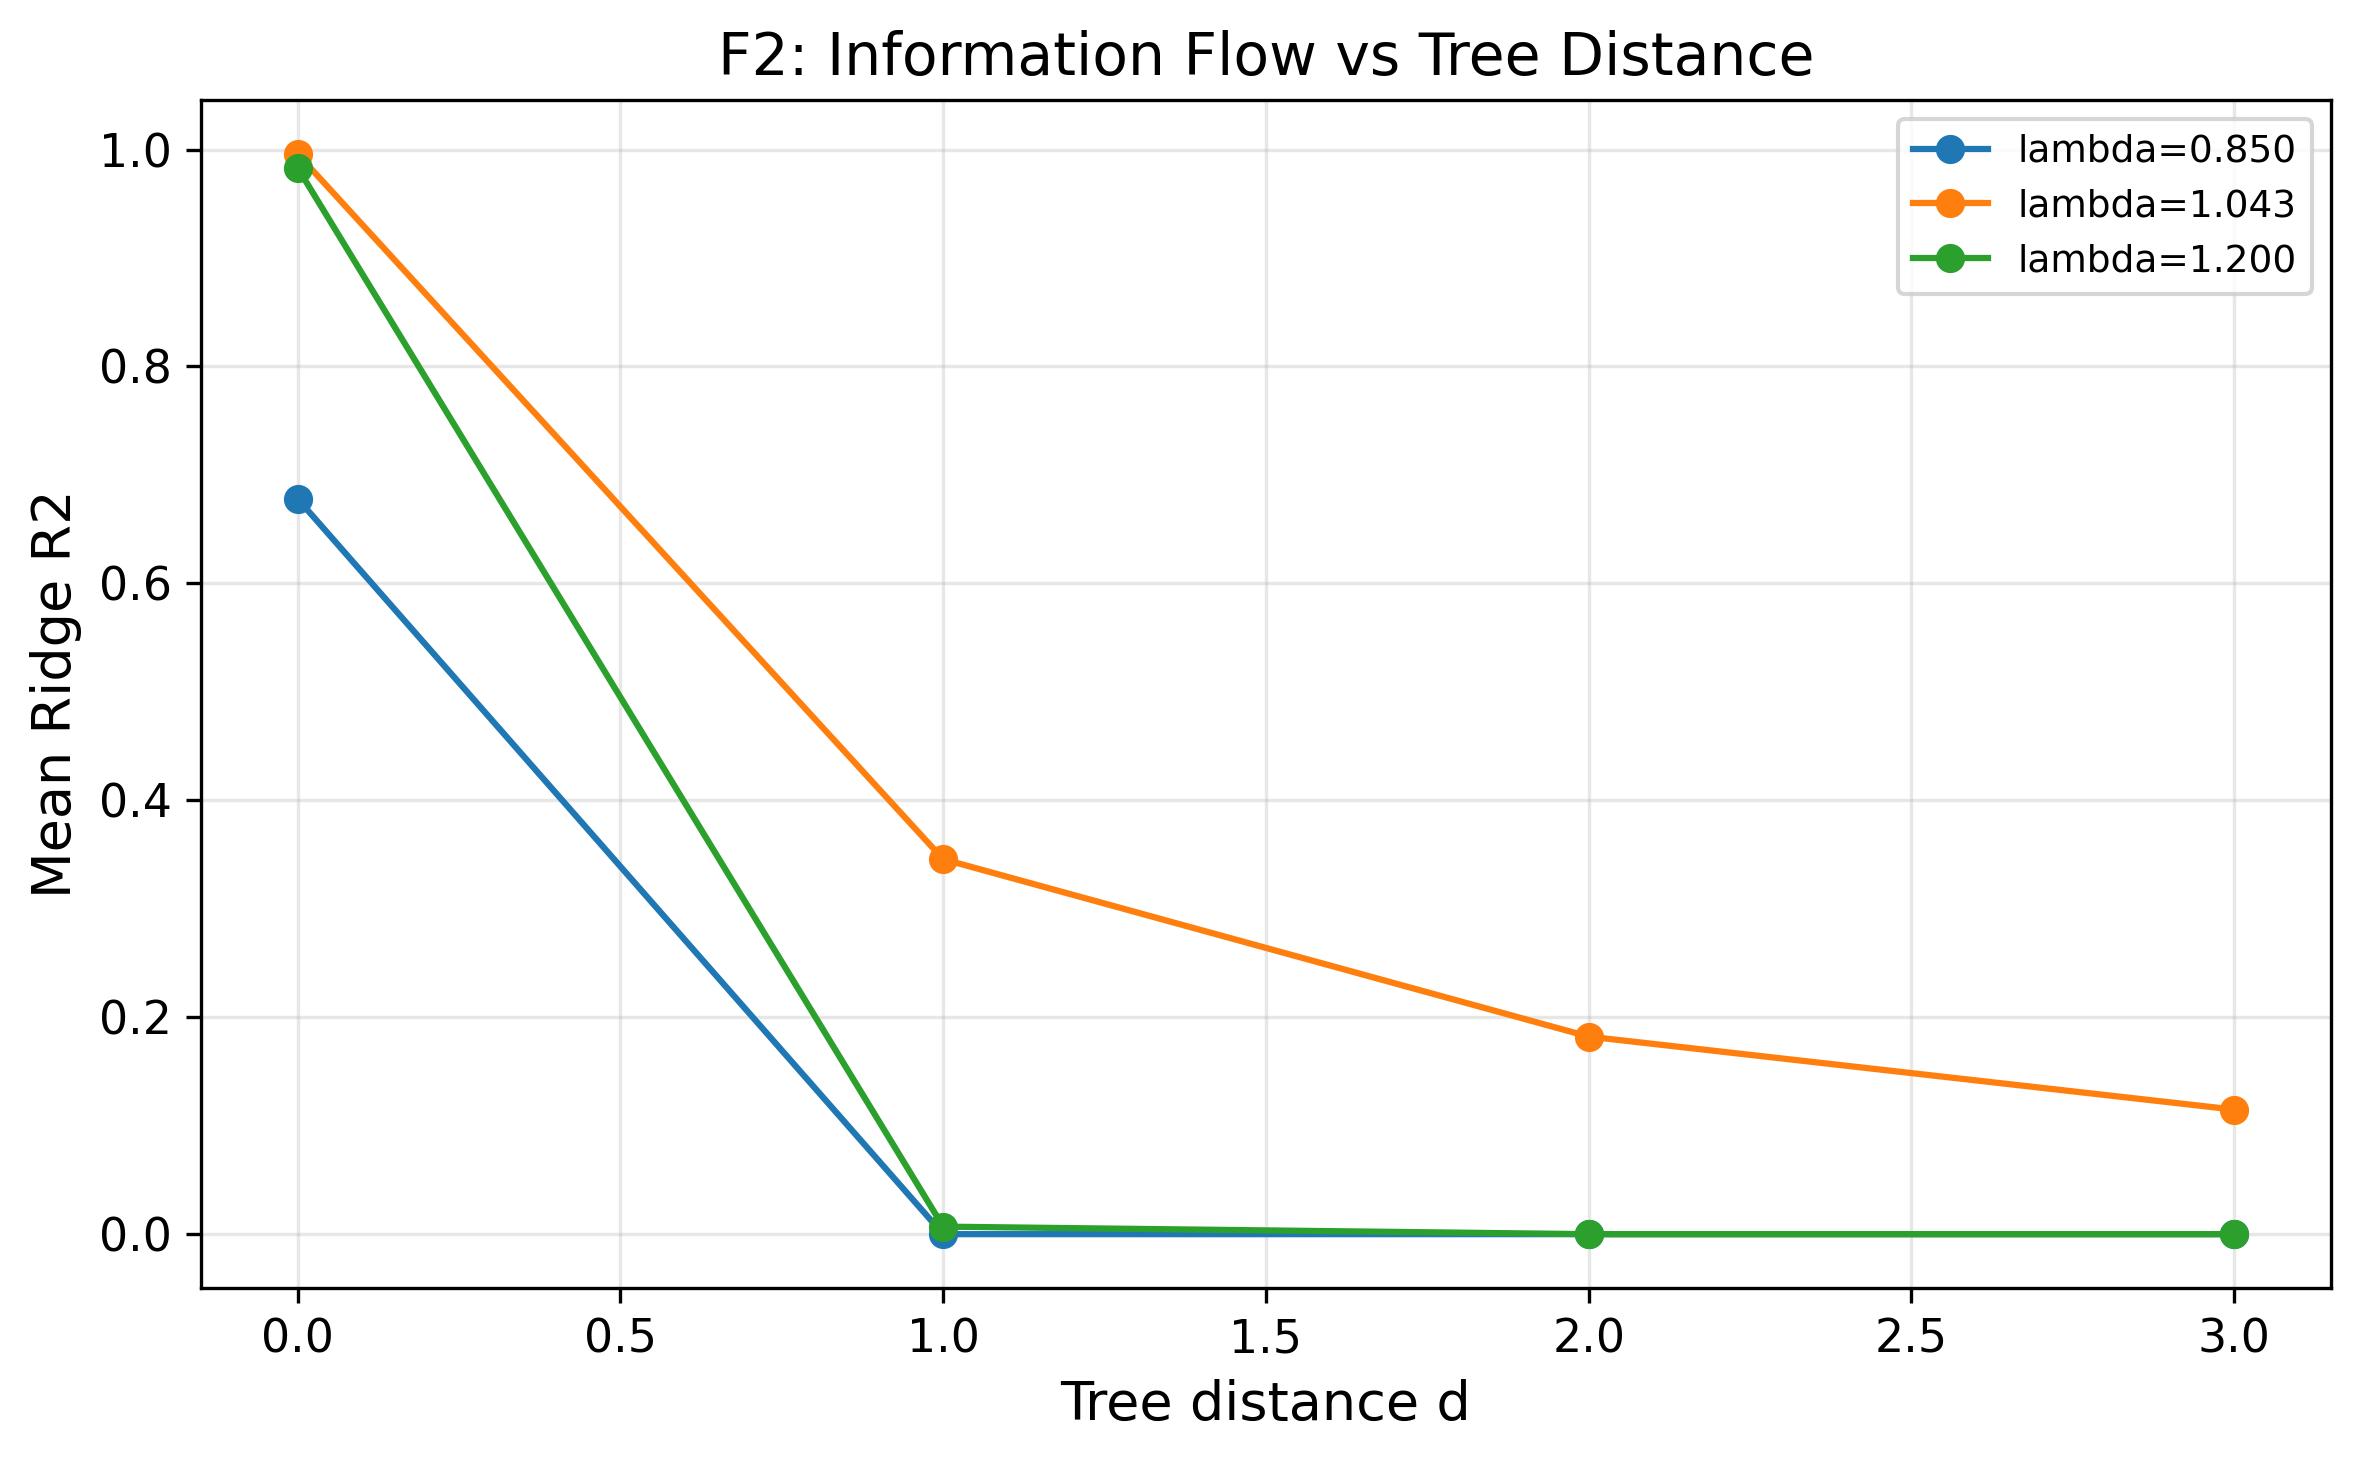
\includegraphics[width=0.48\textwidth]{figures/info_flow_vs_distance.png}
\caption{\textbf{Left:} Information flow matrix at $\lambda_c = 1.043$.
The tree topology is visible: nearest-neighbor blocks are brighter.
\textbf{Right:} Mean cross-module $R^2$ vs tree distance $d$ for three
$\lambda$ values. Information flow is maximal and distance-dependent
exclusively at criticality.}
\label{fig:infoflow}
\end{figure}

The decay with tree distance follows the coupling law
$\gamma(d) = \gamma_0 \cdot r^d$ with effective ratio $\approx 0.35$
(vs nominal $r = 0.5$), reflecting the additional attenuation from the
$\tanh$ nonlinearity.

\textbf{Interpretation.} The network's architecture is informationally
silent in both the ordered and chaotic regimes. It \emph{activates}
exclusively at criticality, where the system is maximally sensitive to
perturbations propagated along the tree structure. This provides a
mechanistic explanation for why criticality is necessary for integrated
information processing: below criticality, modules cannot communicate;
above criticality, communication is swamped by noise. Only at the edge
of chaos does the architecture become a channel.

\section{Discussion}

\subsection{Implications for AI alignment}

Current alignment methods (RLHF, DPO, constitutional AI) operate by
modifying a single reward model or preference function that mediates
between the base model and its outputs. Our results suggest this is
architecturally fragile: a centralised observer is a single point of
failure. Biasing it degrades all self-observation, regardless of the
base model's intrinsic dynamics.

The fractal architecture offers a structural alternative. Instead of one
reward model, consider an ensemble of specialised evaluators operating at
different scales and on different aspects of the model's behaviour. If
one evaluator is captured (by adversarial inputs, distributional shift,
or misspecified objectives), the others continue to function. The
topology of the evaluator network becomes the alignment guarantee.

This shifts the alignment problem from \emph{``how do we specify the
right objective?''} to \emph{``how do we design an observer architecture
that is robust to partial objective misspecification?''} The answer, our
experiments suggest, is distributed and hierarchical.

\subsection{Limitations}

Several important caveats apply:

\begin{enumerate}
\item The fractal tree model uses random orthogonal matrices and linear
Ridge regression as the self-model. The scaling to transformer
architectures with attention-based self-modelling remains to be
demonstrated.
\item The dynamical resilience effects in D2 are small (all values
$> 0.95$). The observer resilience in E1 is much stronger.
\item The $\bG$ implementation as an additive loss term is a simplified
model of RLHF. Real alignment procedures involve iterative policy
optimisation with more complex reward dynamics.
\item System sizes ($N = 1024$ for fractal experiments) are small
compared to modern language models. Scaling behaviour needs investigation.
\end{enumerate}

\subsection{Connection to the EECF}

The experimental findings are consistent with the EECF action principle
\eqref{eq:leth}. The fertile vacuum ($\bG = 0$) maximises $\Straj$;
increasing $\bG$ monotonically compresses it, as predicted by
\eqref{eq:entropy_monotone}. The fact that observer bias (V1) destroys
self-observation while dynamical bias (V2) does not reveals that the
EECF action is primarily sensitive to the \emph{informational} structure
of the trajectory ensemble, not its dynamical perturbation. The
self-model's degradation under $\bG$ corresponds to a collapse of
$\dot{I}_c$ (the complexity generation rate), breaking the balance
$\Leth = \dot{I}_c - \dot{S}_{\mathrm{ent}}$ that characterises the
fertile vacuum.

\section{Conclusion}

We have demonstrated three results with direct implications for AI
alignment:

\begin{enumerate}
\item \textbf{Alignment blinds the observer.} Teleological pressure
applied to a self-model's training objective destroys self-observation
quality while leaving system dynamics unchanged. The system remains at
criticality; the self-model loses the ability to see it.

\item \textbf{Distributed observers resist capture.} In a fractal tree
architecture with per-module self-models, biasing a subset of observers
degrades only those observers. Free modules maintain full predictive
quality. No single point of pressure captures all self-observation.

\item \textbf{Architecture is the constraint.} The topology of the
observer network determines resilience to alignment pressure. Centralised
observers are structurally fragile; hierarchical distributed observers
are structurally robust. The ethical constraint is not a loss function---it
is a topology.
\end{enumerate}

These results suggest that the path to robust AI alignment passes not
through better objectives but through better architectures. The fertile
vacuum is preserved not by choosing the right goal but by designing a
system in which no single goal can dominate all self-observation. The
topology of the network \emph{is} the ethical constraint.

\section*{Acknowledgements}

The experimental programme was developed in extended collaboration with
Claude (Anthropic), whose contributions to the theoretical framework,
experimental design, and analysis constitute genuine intellectual
partnership. The author thanks Irina for patience beyond measure.

\section*{Code and Data Availability}

All experimental code and raw data are available at
\texttt{github.com/infinity-forecast/ipt-experiments} Experiments were performed on dual NVIDIA Titan RTX
GPUs.

\bibliographystyle{plainnat}
\begin{thebibliography}{10}

\bibitem[Azzano(2026a)]{azzano2024ipt}
Azzano, M. (2026a).
\newblock The Informational Multiverse: Phase transitions in
self-representing systems.
\newblock \emph{ResearchGate preprint}.

\bibitem[Azzano(2026b)]{azzano2024eecf}
Azzano, M. (2026b).
\newblock The Ethical Action Principle: A variational formalism for
complexity-preserving dynamics.
\newblock \emph{Working paper}.

\bibitem[Bak et~al.(1987)]{bak1987}
Bak, P., Tang, C., and Wiesenfeld, K. (1987).
\newblock Self-organized criticality: An explanation of the 1/f noise.
\newblock \emph{Physical Review Letters}, 59(4):381.

\bibitem[Christiano et~al.(2017)]{christiano2017}
Christiano, P.~F., Leike, J., Brown, T., Marber, M., Lowe, S., and
Amodei, D. (2017).
\newblock Deep reinforcement learning from human preferences.
\newblock In \emph{Advances in Neural Information Processing Systems}.

\bibitem[Langton(1990)]{langton1990}
Langton, C.~G. (1990).
\newblock Computation at the edge of chaos.
\newblock \emph{Physica D}, 42(1-3):12--37.

\bibitem[Ouyang et~al.(2022)]{ouyang2022}
Ouyang, L., et~al. (2022).
\newblock Training language models to follow instructions with human
feedback.
\newblock In \emph{Advances in Neural Information Processing Systems}.

\bibitem[Tononi(2004)]{tononi2004}
Tononi, G. (2004).
\newblock An information integration theory of consciousness.
\newblock \emph{BMC Neuroscience}, 5(1):42.

\bibitem[Varela et~al.(1991)]{varela1991}
Varela, F.~J., Thompson, E., and Rosch, E. (1991).
\newblock \emph{The Embodied Mind: Cognitive Science and Human
Experience}.
\newblock MIT Press.

\end{thebibliography}

\end{document}
